\chapter{Hasil dan Pembahasan}

\section{Hasil Akhir Desain SQR}

\begin{figure}[h]
	\centering
	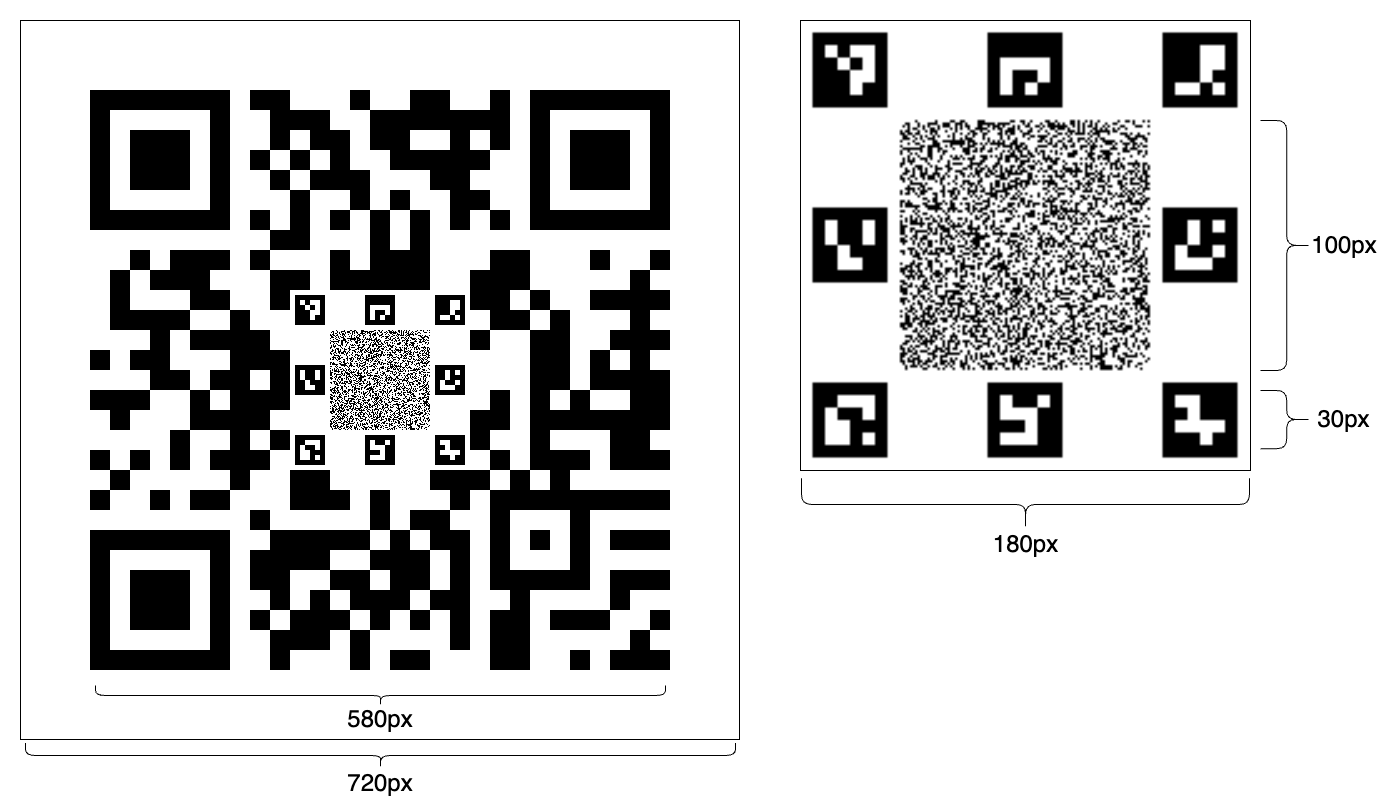
\includegraphics[width=12cm]{contents/chapter-4/4-modelsqrfinal.png}
	\caption{Hasil akhir desain SQR}
	\label{Fig: 4-modelsqrfinal}
\end{figure}

Hasil akhir dari desain SQR yang penulis buat dapat dilihat pada Gambar \ref{Fig: 4-modelsqrfinal}. Versi kode QR yang digunakan adalah kode QR versi 3, dengan
29 modul dan 20 \emph{box-size}, sehingga jika dikalikan ukurannya menjadi 580 x 580 piksel. Selain itu, ditambahkan \emph{padding} berukuran 70 piksel,
sehingga ukuran total dari SQR adalah 720 x 720 piksel. \emph{Watermark} berukuran 180x180 piksel diletakkan di tengah-tengah kode QR. Di dalam
\emph{watermark} tersebut terdapat CDP berukuran 100 x 100 piksel serta delapan penanda ArUco berukuran 28 x 28 piksel. Penanda ArUco yang digunakan adalah
penanda ArUco dengan tipe 4 modul mulai dari id = 0 s.d. id = 7, sehingga lebih mudah dideteksi oleh program karena bentuknya yang relatif lebih sederhana
dibandingkan penanda ArUco yang memiliki ukuran modul lebih tinggi.

\section{Hasil Parameter P\&S}
Hasil parameter yang didapatkan dalam proses P\&S di sini adalah parameter konfigurasi kamera dan jenis kertas maupun tinta yang digunakan untuk mencetak SQR.
\subsection{Konfigurasi Kamera}
Dari eksperimen menggunakan \emph{dataset} pengujian parameter, didapatkan hasil akhir konfigurasi kamera yang digunakan dalam pembuatan \emph{dataset} SQR
orisinal dan palsu yang dapat dilihat pada Tabel \ref{Tab: 4-Parameter Konfigurasi Kamera}.

\begin{table}[!ht]
	\centering
	\caption{Parameter Konfigurasi Kamera}
	\vspace{0.5em}
	\begin{tabular}{|c|c|c|c|}
		\hline
		\textbf{ISO} & \textbf{Shutter Speed} & \textbf{Focus} & \textbf{White Balance} \\ \hline
		200          & 1/100                  & 0,00           & 4000                   \\ \hline
	\end{tabular}
	\label{Tab: 4-Parameter Konfigurasi Kamera}
\end{table}

\noindent Dengan konfigurasi kamera tersebut, 400 \emph{dataset} CDP dapat dilokalisasi dengan baik dari gambar hasil potretan kamera. Lokalisasi yang digunakan sebagai
parameter sukses atau tidaknya adalah lokalisasi menggunakan bantuan penanda ArUco.

Untuk kamera yang digunakan penulis dalam penelitian ini adalah perangkat \emph{smartphone} lain, yaitu Iphone XR dengan konfigurasi kamera yang sama. Hasil
gambar yang dipotret menggunakan Iphone XR dapat dilihat pada Gambar \ref{Fig: 4-hasilfotoiphonexr}.

\begin{figure}[!h]
	\centering
	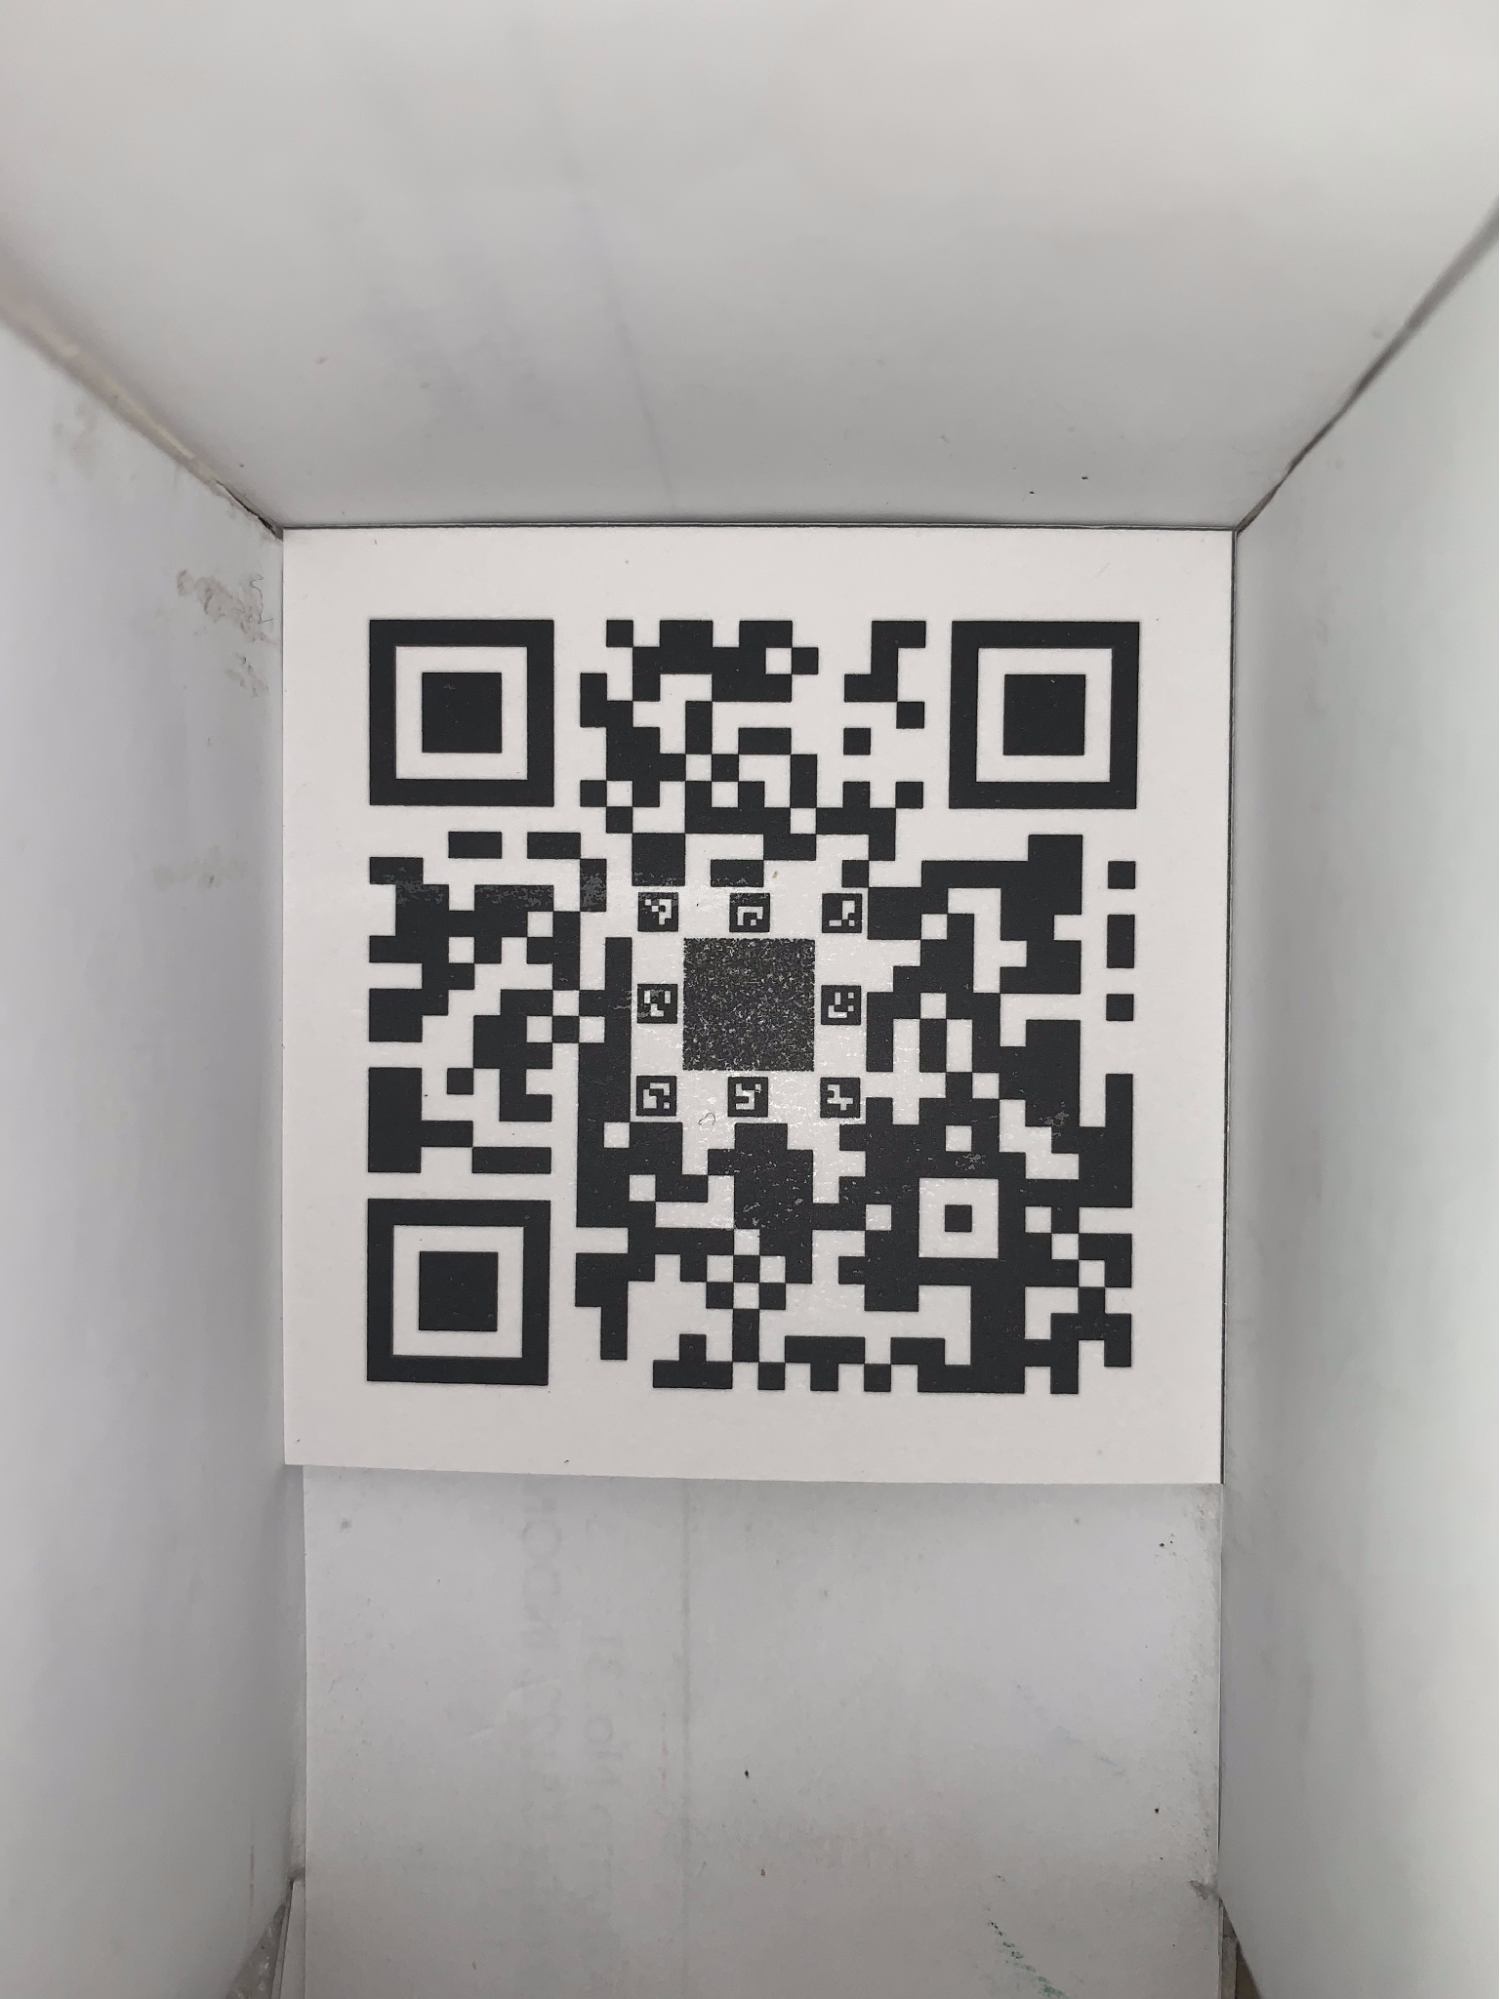
\includegraphics[width=7.5cm]{contents/chapter-4/4-hasilfotoiphonexr.png}
	\caption{Hasil pemotretan SQR menggunakan perangkat Iphone XR}
	\label{Fig: 4-hasilfotoiphonexr}
\end{figure}

\subsection{Jenis Kertas dan Tinta}
Jenis kertas dan tinta yang digunakan dalam pencetakan \emph{dataset} yang penulis gunakan adalah kertas bersifat \emph{doff}, sehingga tidak memantulkan
cahaya dari \emph{flash smarthpone} saat pemotretan berlangsung. Kertas bersifat \emph{doff} yang dapat digunakan seperti \emph{art carton} atau HVS. Opsi lain
adalah dapat menggunakan kertas dan tinta yang bersifat \emph{glossy}, namun diberikan laminasi \emph{doff} di akhir. Pada Gambar \ref{Fig:
	4-perbandingankertas}, dapat dilihat perbedaan hasil pemotretan menggunakan kertas \emph{doff} dan \emph{glossy}, SQR yang dicetak menggunakan kertas dan tinta
\emph{glossy} seperti \emph{ivory} akan memantulkan cahaya, SQR yang dicetak menggunakan kertas dan tinta \emph{doff} seperti \emph{art carton} akan terjaga
kualitasnya karena tidak terkena pantulan cahaya, sedangkan SQR yang dicetak menggunakan kertas dan tinta \emph{glossy} kemudian dilaminasi \emph{doff},
hasilnya baik, namun ada sedikit derau gelembung yang disebabkan oleh proses laminasi.

\begin{figure}[h]
	\centering
	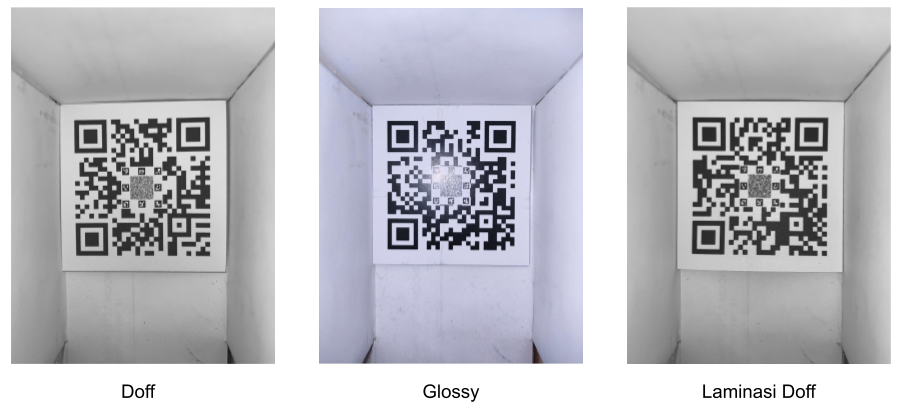
\includegraphics[width=15cm]{contents/chapter-4/4-perbandingankertas.png}
	\caption{Perbandingan gambar hasil pemotretan SQR yang dicetak dengan berbagai tipe kertas}
	\label{Fig: 4-perbandingankertas}
\end{figure}

\section{Hasil Pendeteksian Penanda ArUco}

\begin{table}[h]
	\caption{Tabel hasil pendeteksian penanda ArUco dengan berbagai ukuran}
	\vspace{0.5em}
	\centering
	\begin{tabular}{|c|c|c|}
		\hline
		\textbf{Ukuran ArUco} & \textbf{Jumlah Sukses Terdeteksi} & \textbf{Faktor Penskalaan Terkecil} \\
		\hline
		20                    & 0                                 & -                                   \\
		22                    & 1                                 & 0.3                                 \\
		24                    & 4                                 & 1                                   \\
		26                    & 3                                 & 0.7                                 \\
		28                    & 5                                 & 1                                   \\
		30                    & 5                                 & 1                                   \\
		32                    & 5                                 & 1                                   \\
		34                    & 5                                 & 1                                   \\ \hline
	\end{tabular}
	\label{Tab: 4-tabelhasildeteksiaruco}
\end{table}

Untuk mendapatkan ukuran penanda ArUco yang optimal, penulis menggunakan data uji sejumlah 40 SQR, yang ukuran penanda ArUco-nya berbeda-beda tiap lima SQR,
dari ukuran 20 s.d. 34. Hasil yang didapatkan adalah penanda ArUco dengan ukuran 28 s.d. 34 sukses terdeteksi seluruhnya dengan faktor penskalaan 1, seperti
dapat dilihat pada Tabel \ref{Tab: 4-tabelhasildeteksiaruco}, artinya hasil gambar tidak perlu di-\emph{scaling} untuk mendapatkan hasil deteksi kedelapan
penanda ArUco. Namun, supaya ukuran penanda ArUco tidak terlalu besar, penulis memilih ukuran 28 dan 30 untuk diuji performanya lebih lanjut. Pengujian
selanjutnya adalah menggunakan 40 data untuk masing-masing penanda ArUco berukuran 28 dan 30.

\begin{table}[h]
	\caption{Tabel hasil pendeteksian penanda ArUco dengan berbagai ukuran}
	\vspace{0.5em}
	\centering
	\begin{tabular}{|c|c|c|}
		\hline
		\textbf{Ukuran ArUco} & \textbf{Jumlah Sukses Terdeteksi} & \textbf{Faktor Penskalaan Terkecil} \\
		\hline
		28                    & 40                                & 0.8                                 \\
		30                    & 40                                & 0.9                                 \\ \hline
	\end{tabular}
	\label{Tab: 4-tabelhasildeteksiaruco2}
\end{table}

Hasilnya, seperti dapat dilihat pada Tabel \ref{Tab: 4-tabelhasildeteksiaruco2}, baik penanda ArUco berukuran 28 ataupun 30, semuanya dapat terdeteksi. Karena
hasilnya sama baik, penulis akhirnya memutuskan untuk menggunakan ukuran penanda ArUco yang lebih kecil untuk menghemat ruang yang digunakan pada
\emph{watermark} berukuran 180x180 piksel.

\subsection{Parameter Akhir yang Digunakan}
\noindent Dari hasil verifikasi parameter, berikut adalah parameter pembuatan model SQR:

\begin{itemize}
	\item Ukuran SQR: 580 x 580 piksel
	\item Ukuran SQR beserta \emph{padding}: 720 x 720 piksel
	\item Ukuran \emph{watermark}: 180 x 180 piksel
	\item Ukuran CDP: 100 x 100 piksel
	\item Jumlah penanda ArUco: 8
	\item Ukuran penanda ArUco: 30 x 30 piksel
\end{itemize}

\noindent Untuk parameter P\&S adalah sebagai berikut:
\begin{itemize}
	\item ISO: 200
	\item \emph{Shutter speed}: 1/100
	\item Fokus: 0,00
	\item \emph{White balance}: 4000
	\item Jenis kertas: \emph{Art carton}
	\item Jenis tinta: Tinta buku
\end{itemize}

\section{Deskripsi \emph{Dataset}}
\emph{Dataset} yang digunakan dalam foto SQR sejumlah 400 data dengan rincian: 200 data SQR orisinal 4 level serta 200 data SQR palsu 4 level. \emph{Dataset} tersebut dipotret menggunakan parameter yang telah ditetapkan melalui eksperimen. SQR orisinal merupakan SQR yang dicetak dari format digitalnya, sedangkan SQR palsu di-\emph{generate} dengan menempelkan CDP hasil lokalisasi ke dalam \emph{template} digital kode QR. Contoh sampel data \emph{raw photo} sebelum diolah dapat dilihat pada Gambar \ref{Fig: 4-sampelfotoraw}.

\begin{figure}[!h]
	\centering
	\includegraphics[width=7.5cm]{contents/chapter-4/4-sampelfotoraw.png}
	\caption{Sampel data yang dipotret}
	\label{Fig: 4-sampelfotoraw}
\end{figure}

\section{Analisis Hasil Lokalisasi CDP}
Analisis yang dilakukan adalah mencari interpolasi penskalaan yang memberikan hasil paling mirip dengan \emph{template}, kemudian menganalisis perbandingan
hasil lokalisasi CDP yang menggunakan penanda ArUco (8 titik) dan tanpa menggunakan penanda ArUco (4 titik).
% , dan yang terakhir adalah menganalisis
% karakteristik CDP 2 dan 4 level berdasarkan fitur jarak yang di-\emph{generate}.
\subsection{Analisis Perbandingan Hasil Lokalisasi CDP Orisinal dengan Berbagai Interpolasi Penskalaan}
Sebelum membuat \emph{dataset} SQR palsu, penulis melakukan analisis terhadap \emph{dataset} CDP orisinal hasil lokalisasi. Salah satu analisis yang dilakukan
adalah mencari interpolasi penskalaan yang hasil rata-rata jaraknya dengan \emph{template} paling minimal. Dengan jarak paling kecil, berarti hasil dari
pengolahan data foto pertama dengan interpolasi penskalaan tersebut paling mirip dengan \emph{template}. Hal tersebut menjadi salah satu langkah penyerangan
paling sederhana terhadap CDP orisinal. Hasil rata-rata jarak CDP orisinal dengan template dari masing-masing interpolasi penskalaan dan koefisien jarak dapat
dilihat pada Tabel \ref{Tab: 4-jarakorisinalberbagaiinterpolasi}.

\begin{table}[!ht]
	\centering
	\caption{Hasil rata-rata jarak CDP orisinal dengan \emph{template} dari berbagai interpolasi penskalaan dan koefisien jarak}
	\vspace{0.5em}
	\resizebox{\textwidth}{!}{\begin{tabular}{|l|r|r|r|r|r|}
			\hline
			\multicolumn{1}{|c|}{}  & \multicolumn{1}{c|}{\textbf{INTER\_NEAREST}} & \multicolumn{1}{c|}{\textbf{INTER\_LINEAR}} & \multicolumn{1}{c|}{\textbf{INTER\_AREA}} & \multicolumn{1}{c|}{\textbf{INTER\_CUBIC}} & \multicolumn{1}{c|}{\textbf{INTER\_LANCZOS4}} \\ \hline
			\textbf{sp\_corr}       & 0.8733                                       & \textbf{0.1558}                             & 0.219                                     & 0.1818                                     & 0.1969                                        \\ \hline
			\textbf{sp\_cosine}     & 0.5271                                       & \textbf{0.0708}                             & 0.1751                                    & 0.102                                      & 0.1117                                        \\ \hline
			\textbf{sp\_euclidean}  & 0.7409                                       & \textbf{0.1242}                             & 0.4054                                    & 0.1998                                     & 0.2166                                        \\ \hline
			\textbf{sp\_canberra}   & 0.6098                                       & \textbf{0.1355}                             & 0.5022                                    & 0.239                                      & 0.2464                                        \\ \hline
			\textbf{his\_corr}      & 0.9097                                       & 0.7019                                      & 0.8851                                    & 0.6437                                     & \textbf{0.4568}                               \\ \hline
			\textbf{his\_cosine}    & 0.964                                        & 0.5308                                      & 0.9642                                    & 0.5391                                     & \textbf{0.461}                                \\ \hline
			\textbf{his\_euclidean} & 0.7835                                       & \textbf{0.1689}                             & 0.7843                                    & 0.2045                                     & 0.2023                                        \\ \hline
			\textbf{his\_canberra}  & 0.9329                                       & 0.6476                                      & 0.8123                                    & 0.2149                                     & \textbf{0.1765}                               \\ \hline
			\textbf{dct\_corr}      & 0.4504                                       & \textbf{0.058}                              & 0.1574                                    & 0.0846                                     & 0.0922                                        \\ \hline
			\textbf{dct\_cosine}    & 0.4502                                       & \textbf{0.058}                              & 0.1574                                    & 0.0846                                     & 0.0922                                        \\ \hline
			\textbf{dct\_euclidean} & 0.7326                                       & \textbf{0.1623}                             & 0.4169                                    & 0.2271                                     & 0.2408                                        \\ \hline
			\textbf{dct\_canberra}  & 0.7462                                       & \textbf{0.2985}                             & 0.3739                                    & 0.6722                                     & 0.7312                                        \\ \hline
		\end{tabular}}
	\label{Tab: 4-jarakorisinalberbagaiinterpolasi}
\end{table}

\noindent Dari Tabel \ref{Tab: 4-jarakorisinalberbagaiinterpolasi}, terlihat bahwa interpolasi INTER\_LINEAR merupakan interpolasi penskalaan yang memiliki rata-rata jarak paling minimal, sedangkan INTER\_NEAREST memiliki jarak paling besar. Hal ini menunjukkan CDP hasil lokalisasi dengan interpolasi penskalaan INTER\_LINEAR paling mirip dengan \emph{template}.

Untuk hasil perbandingan secara visual hasil lokalisasi CDP menggunakan berbagai interpolasi penskalaan dapat dilihat pada Gambar x. Terlihat secara kasat mata
bahwa CDP yang dilokalisasi dengan interpolasi penskalaan INTER\_LINEAR memiliki hasil yang lebih mirip dengan \emph{template} dibandingkan dengan yang lain,
terutama CDP yang dilokalisasi dengan interpolasi penskalaan INTER\_NEAREST. Dari hasil tersebut, penulis memutuskan untuk menggunakan interpolasi penskalaan
INTER\_LINEAR dalam pembuatan pemrosesan CDP dan pembuatan \emph{dataset} selanjutnya.

\subsection{Analisis Perbandingan Hasil Lokalisasi CDP menggunakan Penanda ArUco dan Tanpa Penanda ArUco}
Analisis selanjutnya adalah membandingkan hasil lokalisasi CDP menggunakan delapan titik acuan dan empat titik acuan. Delapan titik acuan di sini adalah
delapan penanda ArUco, sedangkan empat titik adalah keempat titik sudut dari kode QR. Analisis yang dilakukan adalah menggunakan koefisien jarak yang mengukur
jarak dari CDP hasil lokalisasi dengan \emph{template}. Hasil lokalisasi yang lebih baik adalah yang jaraknya dengan \emph{template} lebih kecil yang berarti
lebih mirip dengan \emph{template}. Hipotesis awal dari penulis adalah hasil lokalisasi menggunakan 8 titik acuan akan lebih baik daripada 4 titik acuan,
terlebih SQR dipotret pada kondisi permukaan yang tidak rata atau ada lekukan pada sisi-sisi SQR. Koefisien jarak yang digunakan untuk mengukur
kemiripan adalah koefisien jarak korelasi, kosinus, dan \emph{euclidean} dari fitur spasial. Pengujian dilakukan pada \emph{dataset} SQR orisinal dan palsu 4
level. Perbandingan yang dilakukan adalah berdasarkan rata-rata nilai jarak dari grup data.

\begin{table}[!ht]
	\centering
	\caption{Hasil perbandingan rata-rata jarak hasil lokalisasi 8 titik dan 4 titik pada \emph{dataset} CDP orisinal 4 level}
	\vspace{0.5em}
	\begin{tabular}{|l|r|r|}
		\hline
		                       & \multicolumn{1}{c|}{\textbf{8 Titik}} & \multicolumn{1}{c|}{\textbf{4 Titik}} \\ \hline
		\textbf{sp\_corr}      & \textbf{0.3994}                       & 0.8153                                \\ \hline
		\textbf{sp\_cosine}    & \textbf{0.1113}                       & 0.1347                                \\ \hline
		\textbf{sp\_euclidean} & \textbf{27474}                        & 28092                                 \\ \hline
	\end{tabular}
	\label{Tab: 4-jaraklokalisasiarucovsnonarucoori}
\end{table}

Hasil pada data CDP orisinal seperti yang terlihat pada Tabel \ref{Tab: 4-jaraklokalisasiarucovsnonarucoori} menunjukkan bahwa CDP yang dilokalisasi
menggunakan delapan penanda ArUco atau 8 titik memiliki hasil jarak yang lebih kecil. Hal ini menunjukkan bahwa pada data CDP orisinal, lokalisasi menggunakan
8 titik lebih baik daripada 4 titik dalam hal kemiripannya dengan \emph{template}.

\begin{table}[!ht]
	\centering
	\caption{Hasil perbandingan rata-rata jarak hasil lokalisasi 8 titik dan 4 titik pada \emph{dataset} CDP palsu 4 level}
	\vspace{0.5em}
	\begin{tabular}{|l|r|r|}
		\hline
		                       & \multicolumn{1}{l|}{\textbf{8 titik}} & \multicolumn{1}{l|}{\textbf{4 titik}} \\ \hline
		\textbf{sp\_corr}      & \textbf{0.6147}                       & 0.8749                                \\ \hline
		\textbf{sp\_cosine}    & \textbf{0.108}                        & 0.1382                                \\ \hline
		\textbf{sp\_euclidean} & \textbf{27797}                        & 29880                                 \\ \hline
	\end{tabular}
	\label{Tab: 4-jaraklokalisasiarucovsnonarucopalsu}
\end{table}

Hasil yang sama juga didapat pada CDP palsu, CDP yang dilokalisasi menggunakan delapan penanda ArUco atau 8 titik memiliki hasil jarak yang lebih kecil. Hal
ini menunjukkan bahwa pada data CDP palsu, lokalisasi menggunakan 8 titik lebih baik daripada 4 titik dalam hal kemiripannya dengan \emph{template}. Untuk
perbandingan visual salah satu hasil lokalisasi CDP menggunakan 4 titik dan 8 titik dapat dilihat pada Gambar \ref{Fig: 4-cdplokalisasi8vs4}. Terlihat bahwa
hasil lokalisasi CDP menggunakan 4 titik kurang rapi, ada celah kosong di atasnya yang bukan merupakan komponen CDP itu sendiri. Selain itu, hasil lokalisasi
CDP menggunakan 4 titik terlihat lebih kabur. Hal tersebut dapat disebabkan ada lekukan pada data SQR yang dipotret. Hasil lokalisasi CDP menggunakan 8
titik terlihat jauh lebih rapi pada perbandingan tersebut.

\begin{figure}[h]
	\centering
	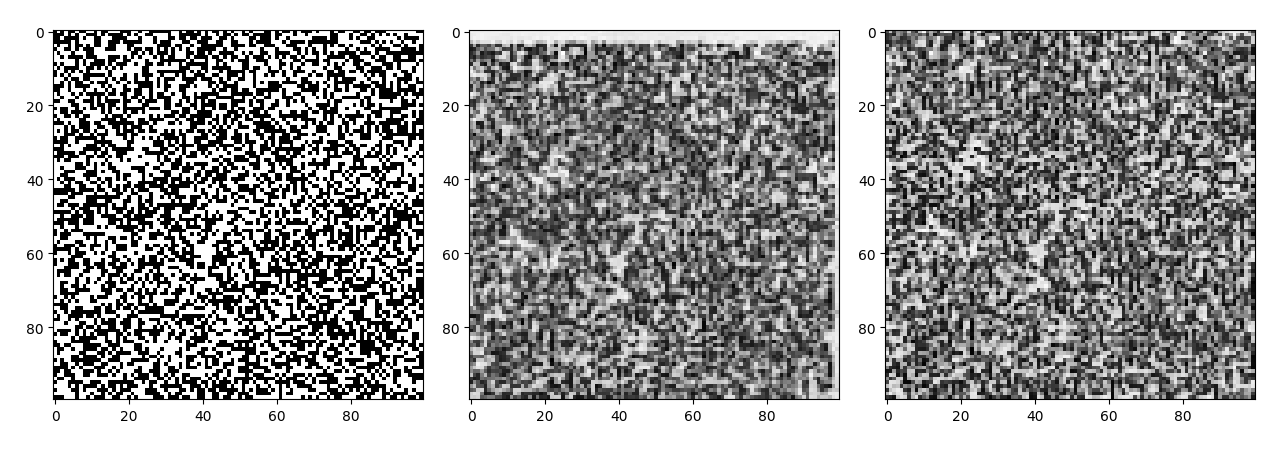
\includegraphics[width=12cm]{contents/chapter-4/4-cdplokalisasi8vs4_2.png}
	\caption{Perbandingan CDP \emph{template} dengan yang dilokalisasi dengan 4 titik (tengah) dan CDP yang dilokalisasi dengan 8 titik (kanan)}
	\label{Fig: 4-cdplokalisasi8vs4}
\end{figure}

Dari kedua pengujian pada CDP orisinal dan CDP palsu, dapat disimpulkan bahwa lokalisasi CDP menggunakan delapan penanda ArUco menghasilkan hasil lokalisasi
yang lebih baik dalam hal kemiripannya dengan \emph{template}. Hal tersebut tentunya akan berpengaruh dalam akurasi model yang akan dibuat, karena data CDP
yang diproses lebih berkualitas.

% \subsection{Perbandingan Hasil CDP \emph{Template}, Orisinal, dan Palsu}
% \subsection{Analisis Signifikansi CDP 2 dan 4 Level}
% \begin{table}[!h]
% 	\centering
% 	\caption{Hasil pengujian \emph{T-test} pada data grup fitur jarak CDP 2 level dengan data grup fitur jarak CDP 4 level}
% 	\vspace{0.5em}
% 	\begin{tabular}{|l|rr|rr|}
% 		\hline
% 		\multirow{2}{*}{}       & \multicolumn{2}{c|}{\textbf{Orisinal}}    & \multicolumn{2}{c|}{\textbf{Palsu}}                                                                                       \\ \cline{2-5}
% 		                        & \multicolumn{1}{c|}{\textbf{T-statistic}} & \multicolumn{1}{c|}{\textbf{P-value}} & \multicolumn{1}{c|}{\textbf{T-statistic}} & \multicolumn{1}{c|}{\textbf{P-value}} \\ \hline
% 		\textbf{sp\_corr}       & \multicolumn{1}{r|}{-16.7459}             & 5.01E-48                              & \multicolumn{1}{r|}{-15.4077}             & 2.42E-42                              \\ \hline
% 		\textbf{sp\_cosine}     & \multicolumn{1}{r|}{2.6649}               & 0.008014430587                        & \multicolumn{1}{r|}{5.6064}               & 3.87E-08                              \\ \hline
% 		\textbf{sp\_euclidean}  & \multicolumn{1}{r|}{18.6804}              & 2.27E-56                              & \multicolumn{1}{r|}{15.9246}              & 1.59E-44                              \\ \hline
% 		\textbf{sp\_canberra}   & \multicolumn{1}{r|}{13.5024}              & 1.81E-34                              & \multicolumn{1}{r|}{17.1141}              & 1.32E-49                              \\ \hline
% 		\textbf{his\_corr}      & \multicolumn{1}{r|}{34.4186}              & 2.31E-121                             & \multicolumn{1}{r|}{22.146}               & 2.13E-71                              \\ \hline
% 		\textbf{his\_cosine}    & \multicolumn{1}{r|}{77.323}               & 7.51E-242                             & \multicolumn{1}{r|}{69.1668}              & 6.46E-224                             \\ \hline
% 		\textbf{his\_euclidean} & \multicolumn{1}{r|}{43.2212}              & 2.09E-152                             & \multicolumn{1}{r|}{43.7259}              & 4.60E-154                             \\ \hline
% 		\textbf{his\_canberra}  & \multicolumn{1}{r|}{132.6975}             & 0                                     & \multicolumn{1}{r|}{88.0526}              & 4.52E-263                             \\ \hline
% 		\textbf{dct\_corr}      & \multicolumn{1}{r|}{4.2178}               & 3.06E-05                              & \multicolumn{1}{r|}{6.5174}               & 2.17E-10                              \\ \hline
% 		\textbf{dct\_cosine}    & \multicolumn{1}{r|}{4.213}                & 3.12E-05                              & \multicolumn{1}{r|}{6.5082}               & 2.29E-10                              \\ \hline
% 		\textbf{dct\_euclidean} & \multicolumn{1}{r|}{14.0464}              & 1.10E-36                              & \multicolumn{1}{r|}{9.6896}               & 4.49E-20                              \\ \hline
% 		\textbf{dct\_canberra}  & \multicolumn{1}{r|}{-3.4369}              & 0.0006503627876                       & \multicolumn{1}{r|}{6.8627}               & 2.60E-11                              \\ \hline
% 	\end{tabular}
% 	\label{Tab: 4-hasilujisignifikansi2vs4level}
% \end{table}

% Analisis ini digunakan untuk mengetahui apakah ada perbedaan karakteristik yang mencolok antara CDP 2 dan 4 level, baik orisinal maupun palsu, diukur dari
% jaraknya dengan \emph{template}. Analisis dilakukan dengan melakukan uji statistik \emph{T-test} untuk menguji signifikansi antara data kelompok CDP orisinal 2
% dan 4 level dan juga CDP palsu 2 dan 4 level. Selain itu, dilakukan visualisasi plot distribusi untuk melihat secara visual karakteristik dan perbedaan dari
% kedua data grup berdasarkan jaraknya dengan \emph{template} untuk tiap-tiap koefisien jarak.

% Dari Tabel \ref{Tab: 4-hasilujisignifikansi2vs4level} terlihat bahwa hasilnya adalah signifikan untuk seluruh koefisien jarak, baik pada \emph{dataset} CDP
% orisinal dan palsu. Dua grup dapat dikatakan signifikan perbedaannya apabila memiliki \emph{P-value} < 0,05 (diambil dari nilai \emph{P-value} yang sering
% digunakan). Semakin kecil nilai \emph{P-value}, semakin signifikan perbedaan antara dua grup data. Dari Tabel \ref{Tab: 4-hasilujisignifikansi2vs4level} dapat
% dilihat bahwa koefisien jarak yang memiliki signifikansi tertinggi dalam membedakan kedua data grup adalah \emph{his\_canberra}, \emph{his\_cosine},
% \emph{his\_euclidean}, dan \emph{his\_corr}.

% Selain itu, untuk memudahkan melihat signifikansi antara kedua data grup secara visual, penulis melakukan plot distribusi untuk tiap-tiap koefisien jarak.
% Untuk hasil plot distribusi \emph{dataset} CDP orisinal dapat dilihat pada \ref{Fig: 4-ori2levelvsori4level}. Terlihat bahwa fitur histogram dapat memisahkan
% CDP 2 dan 4 level orisinal dengan baik. Hal ini sesuai dengan hasil pengujian statistik \emph{T-test} dengan empat peringkat teratas untuk jarak yang memiliki
% perbedaan paling signifikan, memisahkan 2 dan 4 level adalah \emph{his\_canberra}, \emph{his\_cosine}, \emph{his\_euclidean}, dan \emph{his\_corr}. Hasil lain
% yang diperoleh adalah CDP 4 level memiliki jarak yang lebih dekat dengan \emph{template} dibandingkan dengan CDP 2 level. Hal ini menunjukkan bahwa CDP 4 level
% lebih sulit terdegradasi melalui proses P\&S dibandingkan CDP 2 level.

% Selanjutnya untuk hasil plot distribusi \emph{dataset} CDP palsu dapat dilihat pada \ref{Fig: 4-fake2levelvsfake4level}. Terlihat bahwa hasilnya mirip bahkan
% hampir sama dengan plot distribusi pada \emph{dataset} CDP orisinal. Fitur histogram mampu memisahkan CDP 2 dan 4 level dengan baik. CDP 4 level juga memiliki
% jarak yang lebih dekat dengan \emph{template} dibandingkan dengan CDP 2 level. Analisis selanjutnya adalah melihat signifikansi antara CDP orisinal dan palsu
% berdasarkan fitur jaraknya.

% \clearpage

% \begin{figure}[!ht]
% 	\centering
% 	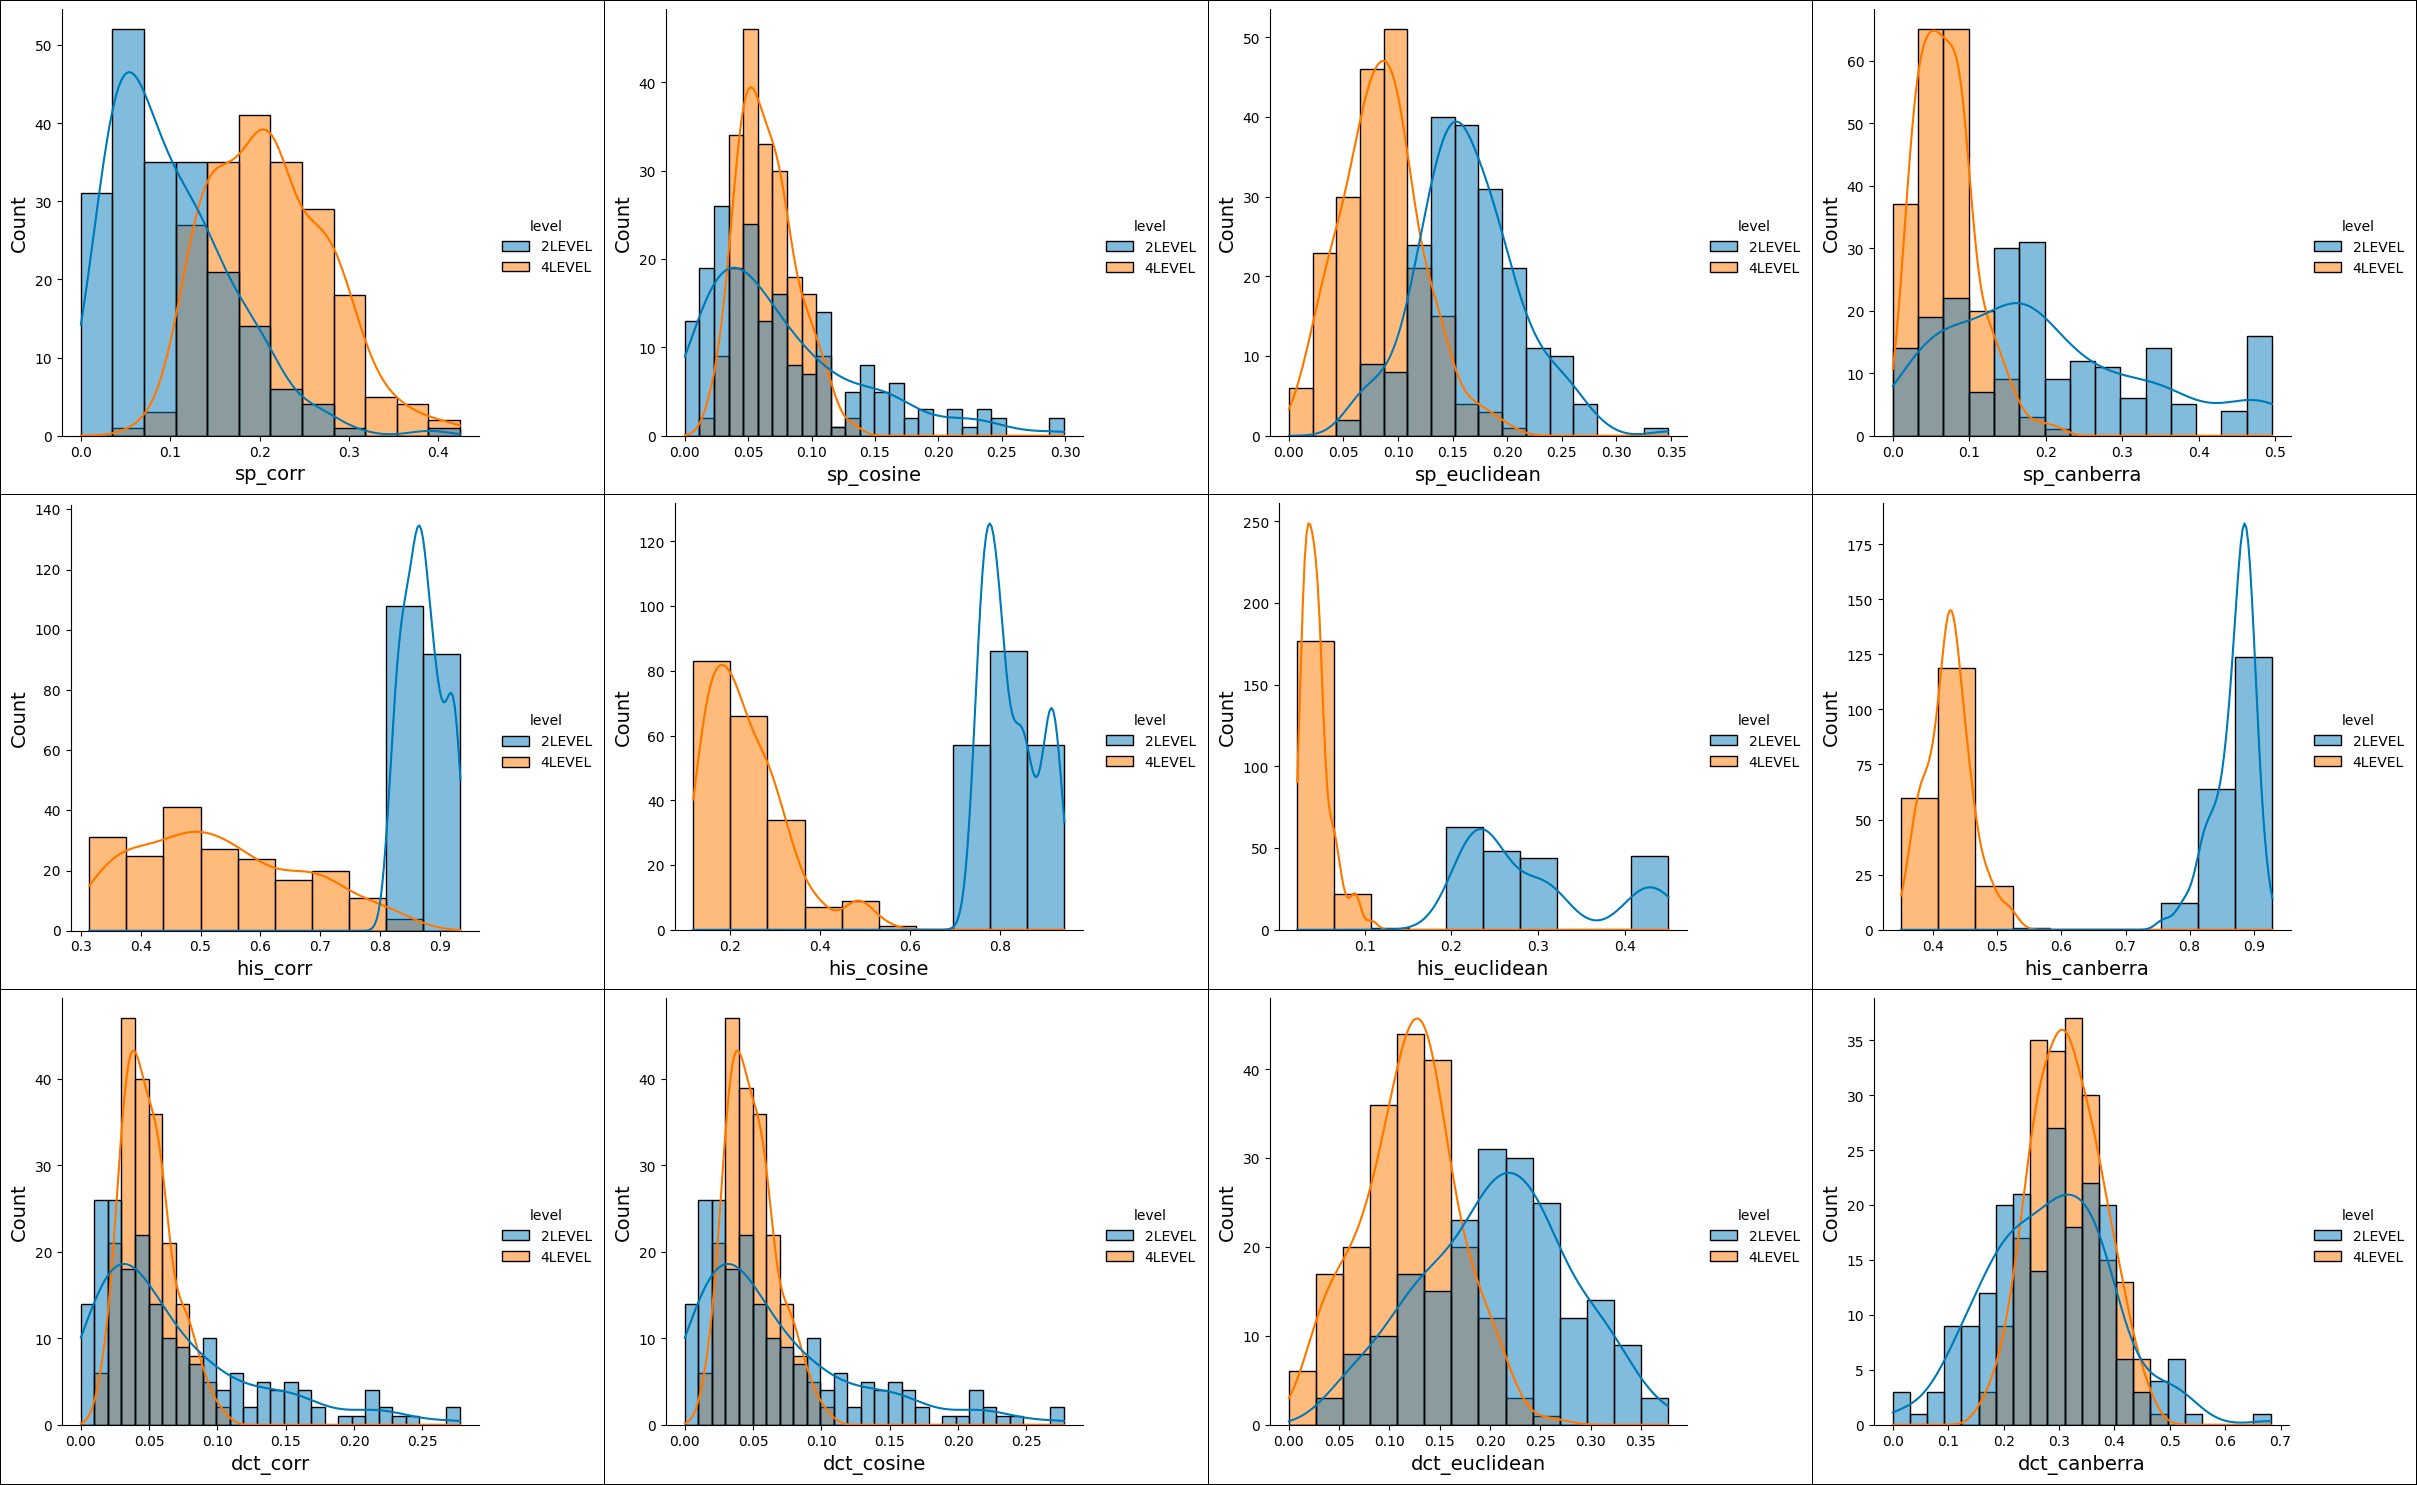
\includegraphics[width=\textwidth]{contents/chapter-4/4-ori2levelvsori4level.png}
% 	\caption{Plot distribusi koefisien jarak CDP orisinal 2 dan 4 level}
% 	\label{Fig: 4-ori2levelvsori4level}
% \end{figure}

% \begin{figure}[!ht]
% 	\centering
% 	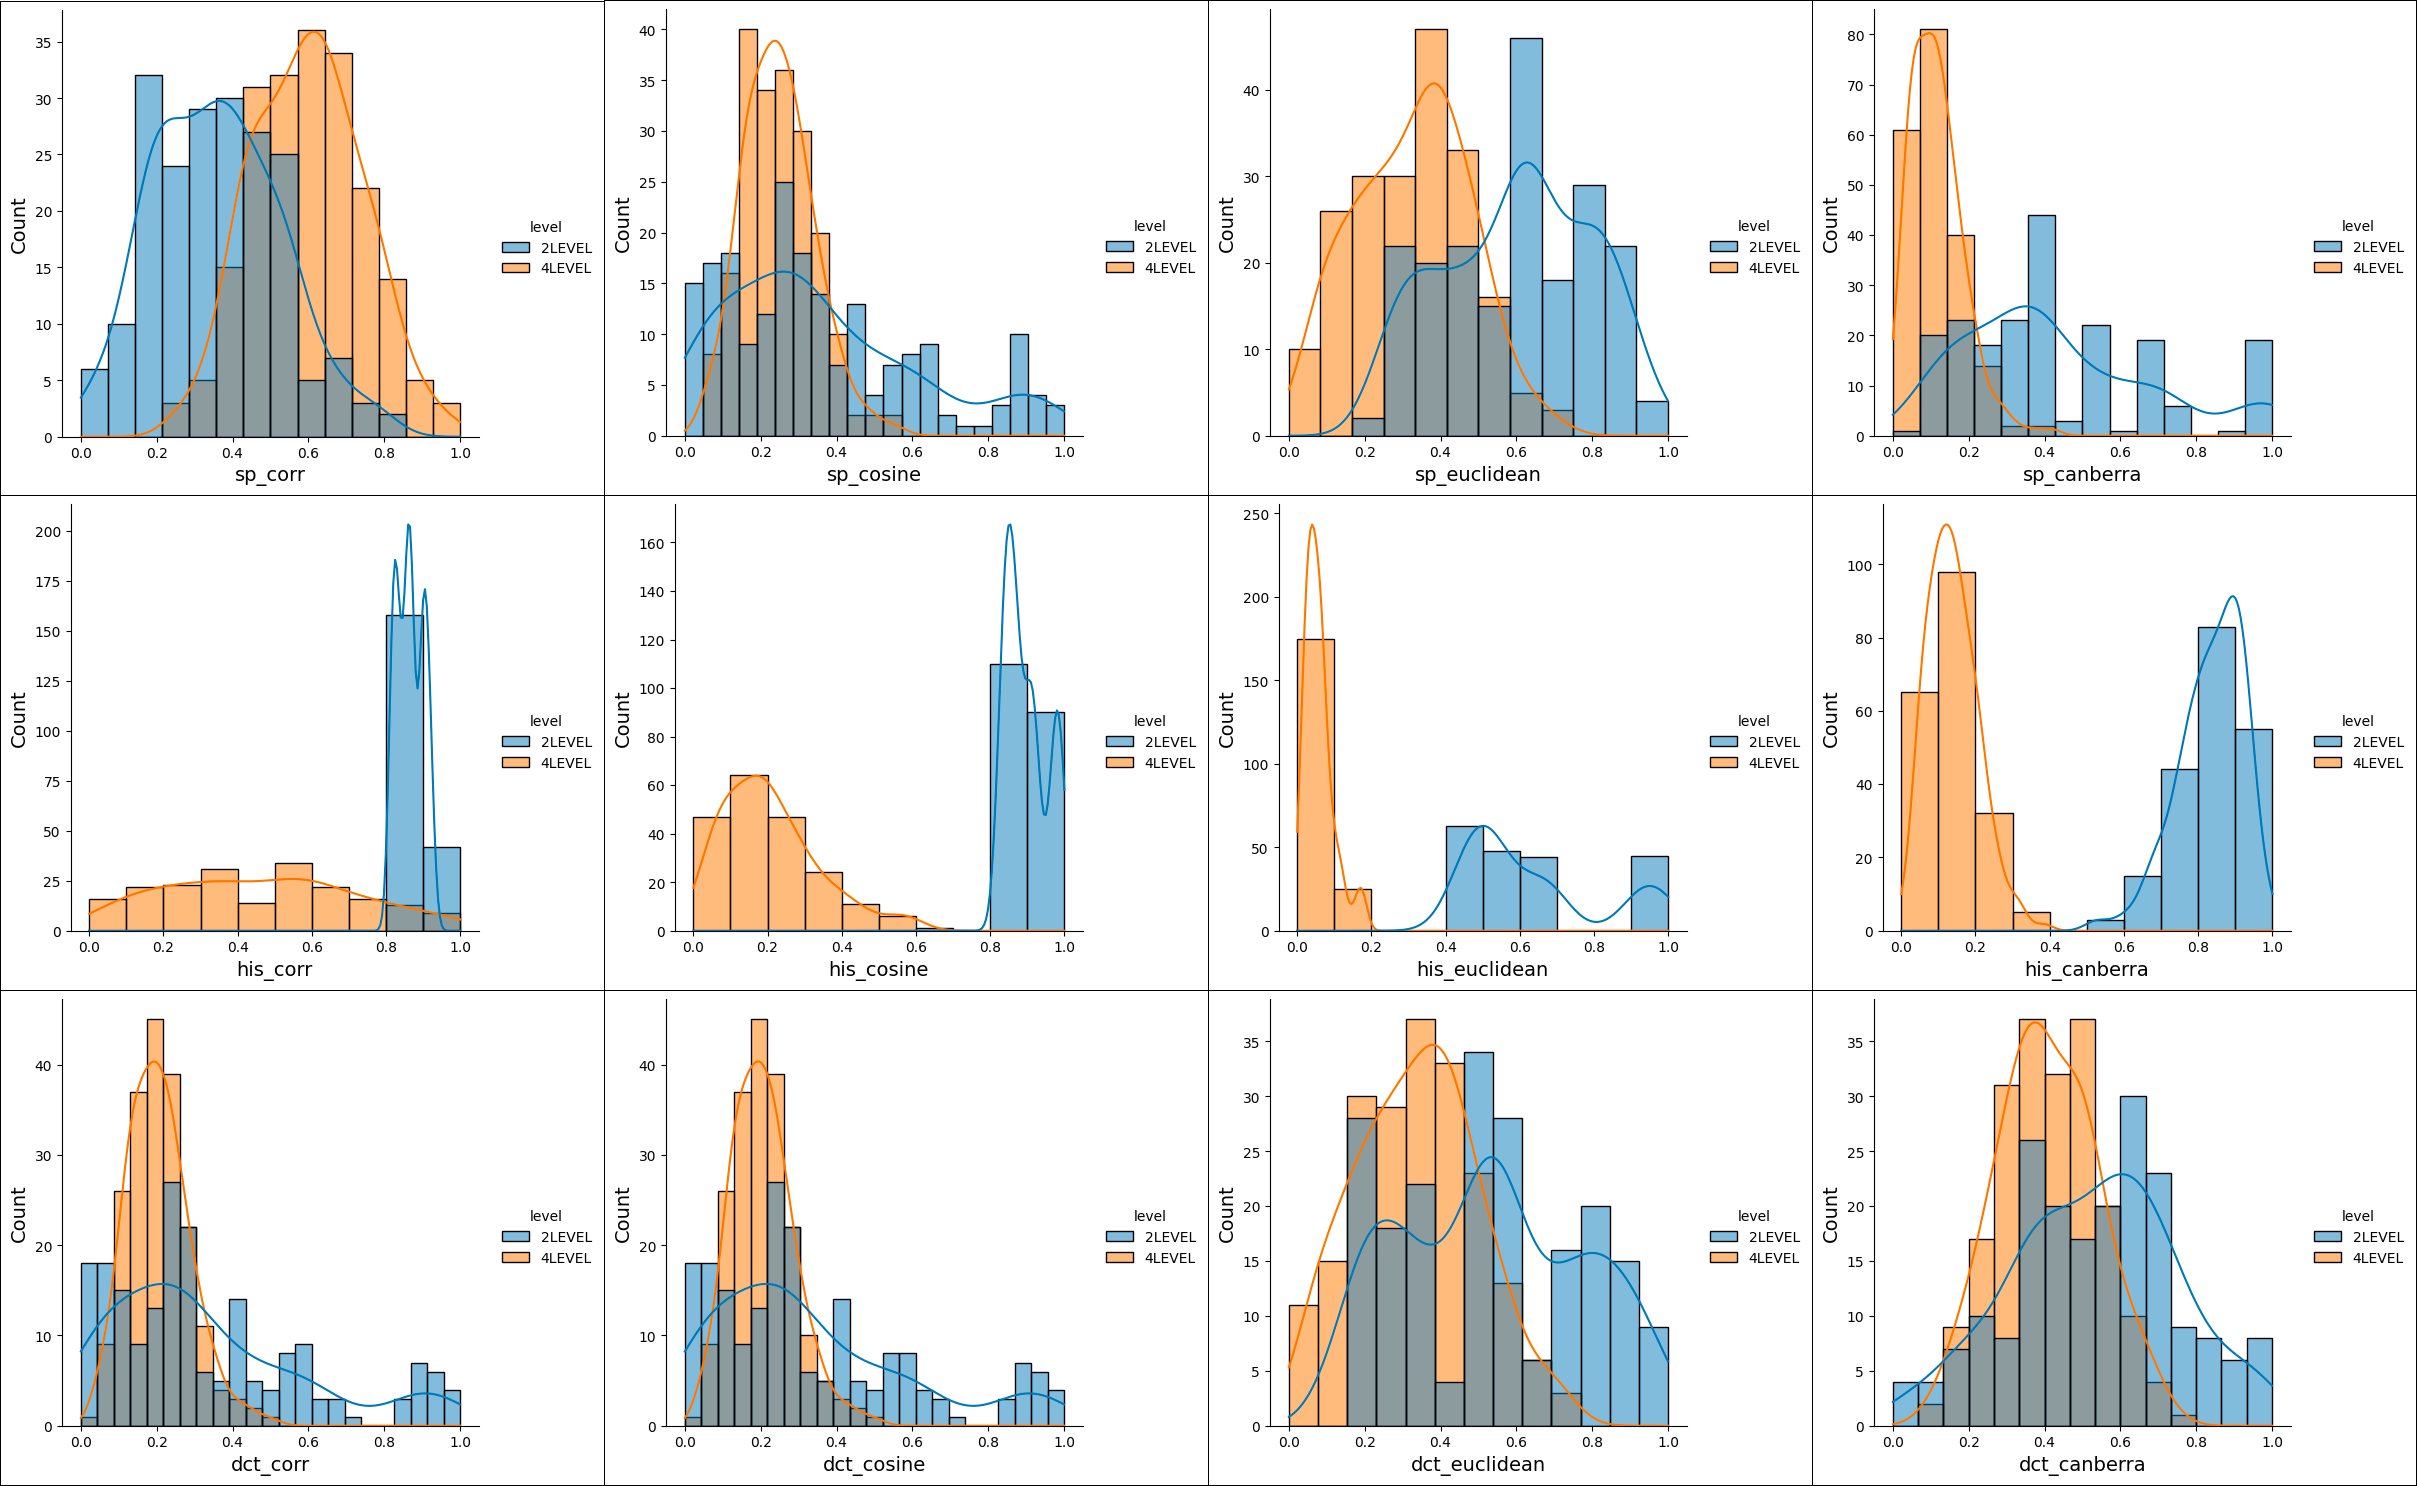
\includegraphics[width=\textwidth]{contents/chapter-4/4-fake2levelvsfake4level.png}
% 	\caption{Plot distribusi koefisien jarak CDP palsu 2 dan 4 level}
% 	\label{Fig: 4-fake2levelvsfake4level}
% \end{figure}

% \clearpage

\subsection{Analisis Signifikansi CDP Orisinal dan Palsu}
Analisis ini digunakan untuk mengetahui apakah ada perbedaan karakteristik yang mencolok antara CDP orisinal dan palsu, baik yang dilokalisasi menggunakan
penanda ArUco (8 titik) maupun yang dilokalisasi tanpa menggunakan penanda ArUco (4 titik). Analisis dilakukan dengan melakukan uji statistik \emph{T-test}
untuk menguji signifikansi antara data kelompok CDP orisinal dengan CDP palsu. Selain itu, dilakukan visualisasi plot distribusi untuk melihat secara visual
karakteristik dan perbedaan dari kedua data grup berdasarkan jaraknya dengan \emph{template} untuk tiap-tiap koefisien jarak.

% baik 2 level maupun 4 level, diukur dari jaraknya dengan \emph{template}. Analisis dilakukan dengan melakukan uji statistik \emph{T-test} untuk menguji
% signifikansi antara data kelompok CDP 2 level orisinal dan palsu dan juga CDP 4 level orisinal dan palsu. Selain itu, dilakukan visualisasi plot distribusi
% untuk melihat secara visual karakteristik dan perbedaan dari kedua data grup berdasarkan jaraknya dengan \emph{template} untuk tiap-tiap koefisien jarak.

\begin{table}[h]
	\centering
	\caption{Hasil pengujian \emph{T-test} pada data grup fitur jarak CDP orisinal dengan palsu, pada CDP yang dilokalisasi dengan 8 titik dan CDP yang dilokalisasi dengan 4 titik}
	\vspace{0.5em}
	\begin{tabular}{|l|rr|rr|}
		\hline
		\multirow{2}{*}{}       & \multicolumn{2}{c|}{\textbf{8 Titik}}     & \multicolumn{2}{c|}{\textbf{4 Titik}}                                                                                     \\ \cline{2-5}
		                        & \multicolumn{1}{c|}{\textbf{T-statistic}} & \multicolumn{1}{c|}{\textbf{P-value}} & \multicolumn{1}{c|}{\textbf{T-statistic}} & \multicolumn{1}{c|}{\textbf{P-value}} \\ \hline
		\textbf{sp\_corr}       & \multicolumn{1}{r|}{-56.5046}             & 3.32E-192                             & \multicolumn{1}{r|}{-4.3128}              & 2.04E-05                              \\ \hline
		\textbf{sp\_cosine}     & \multicolumn{1}{r|}{-32.3355}             & 2.08E-113                             & \multicolumn{1}{r|}{-0.8523}              & 0.3945606046                          \\ \hline
		\textbf{sp\_euclidean}  & \multicolumn{1}{r|}{-39.9488}             & 2.43E-141                             & \multicolumn{1}{r|}{-5.4538}              & 8.67E-08                              \\ \hline
		\textbf{sp\_canberra}   & \multicolumn{1}{r|}{-33.0441}             & 3.86E-116                             & \multicolumn{1}{r|}{-5.19}                & 3.36E-07                              \\ \hline
		\textbf{his\_corr}      & \multicolumn{1}{r|}{-6.0236}              & 3.89E-09                              & \multicolumn{1}{r|}{-6.0636}              & 3.10E-09                              \\ \hline
		\textbf{his\_cosine}    & \multicolumn{1}{r|}{-7.7801}              & 6.30E-14                              & \multicolumn{1}{r|}{-10.7008}             & 1.17E-23                              \\ \hline
		\textbf{his\_euclidean} & \multicolumn{1}{r|}{-6.6484}              & 9.79E-11                              & \multicolumn{1}{r|}{-11.2637}             & 9.84E-26                              \\ \hline
		\textbf{his\_canberra}  & \multicolumn{1}{r|}{-24.5923}             & 7.04E-82                              & \multicolumn{1}{r|}{-26.4865}             & 7.49E-90                              \\ \hline
		\textbf{dct\_corr}      & \multicolumn{1}{r|}{-29.4935}             & 3.53E-102                             & \multicolumn{1}{r|}{-1.2032}              & 0.2296019564                          \\ \hline
		\textbf{dct\_cosine}    & \multicolumn{1}{r|}{-29.5221}             & 2.71E-102                             & \multicolumn{1}{r|}{-1.2216}              & 0.2225752757                          \\ \hline
		\textbf{dct\_euclidean} & \multicolumn{1}{r|}{-29.7315}             & 3.90E-103                             & \multicolumn{1}{r|}{-8.8239}              & 3.53E-17                              \\ \hline
		\textbf{dct\_canberra}  & \multicolumn{1}{r|}{-55.4671}             & 2.32E-189                             & \multicolumn{1}{r|}{-7.6051}              & 2.07E-13                              \\ \hline
	\end{tabular}
	\label{Tab: 4-hasilujisignifikansiorivspalsu}
\end{table}

Dari Tabel \ref{Tab: 4-hasilujisignifikansiorivspalsu} terlihat bahwa dengan menggunakan nilai \emph{P-value} = 0,5, pada CDP yang dilokalisasi menggunakan 8
titik, seluruh fitur dapat dikatakan signifikan antara CDP orisinal dengan CDP palsunya. Namun, pada CDP yang dilokalisasi menggunakan 4 titik, ada yang
nilainya tidak signifikan, yaitu pada fitur jarak \emph{sp\_cosine}, \emph{dct\_corr}, dan \emph{dct\_cosine}. Selain itu, level signifikansinya juga berbeda
jauh antara CDP yang dilokalisasi dengan 8 titik dan CDP yang dilokalisasi dengan 4 titik. CDP yang dilokalisasi dengan 8 titik memiliki signifikansi yang jauh
lebih tinggi, terlihat dari kecilnya \emph{P-value} yang didapat pada masing-masing koefisien jarak.

% pada CDP 2 level, ada 2 fitur jarak yang
% tidak signifikan antara CDP orisinal dan palsunya, yaitu \emph{his\_corr} dan \emph{his\_euclidean}. Pada CDP 4 level, dengan nilai \emph{P-value} yang sama,
% seluruh fitur jarak dapat dikatakan signifikan antara CDP orisinal dan palsunya. Dari Tabel \ref{Tab: 4-hasilujisignifikansiorivspalsu} dapat dilihat bahwa
% baik CDP 2 dan 4 level, koefisien jarak yang memiliki nilai paling signifikan antara orisinal dan palsu adalah \emph{sp\_corr}, disusul \emph{dct\_canberra},
% dan \emph{sp\_euclidean}.

Selain itu, untuk memudahkan melihat signifikansi antara kedua data grup secara visual, penulis melakukan plot distribusi untuk tiap-tiap koefisien jarak.
Untuk hasil plot distribusi \emph{dataset} CDP yang dilokalisasi dengan 8 titik dan \emph{dataset} CDP yang dilokalisasi dengan 4 titik dapat dilihat pada
Gambar \ref{Fig: 4-4levelorivs4levelfake} dan \ref{Fig: 4-orivsfake4titik}. Hasilnya sangat terlihat bahwa pada \emph{dataset} CDP yang dilokalisasi dengan 8
titik, distribusi antara CDP orisinal dengan palsunya dapat terpisahkan dengan baik, sedangkan pada \emph{dataset} CDP yang dilokalisasi dengan 4 titik,
distribusi antara CDP orisinal dengan palsunya tidak terpisahkan dengan baik, terlihat dari banyaknya \emph{overlap}. Hal tersebut menunjukkan bahwa CDP yang
dilokalisasi dengan 8 titik mendapatkan fitur yang signifikansi antara CDP orisinal dengan palsunya sangat tinggi.

% CDP 2 level dapat dilihat pada \ref{Fig: 4-2levelorivs2levelfake}. Terlihat bahwa pada \emph{dataset} CDP 2 level,
% fitur terbaik yang memisahkan CDP orisinal dan palsu adalah \emph{sp\_corr}. Selain itu, fitur spasial yang lain juga memiliki signifikansi yang tinggi. Selain
% itu, ada fitur \emph{dct\_canberra} yang juga memiliki signifikansi yang tinggi.

% \begin{figure}[!h]
% 	\centering
% 	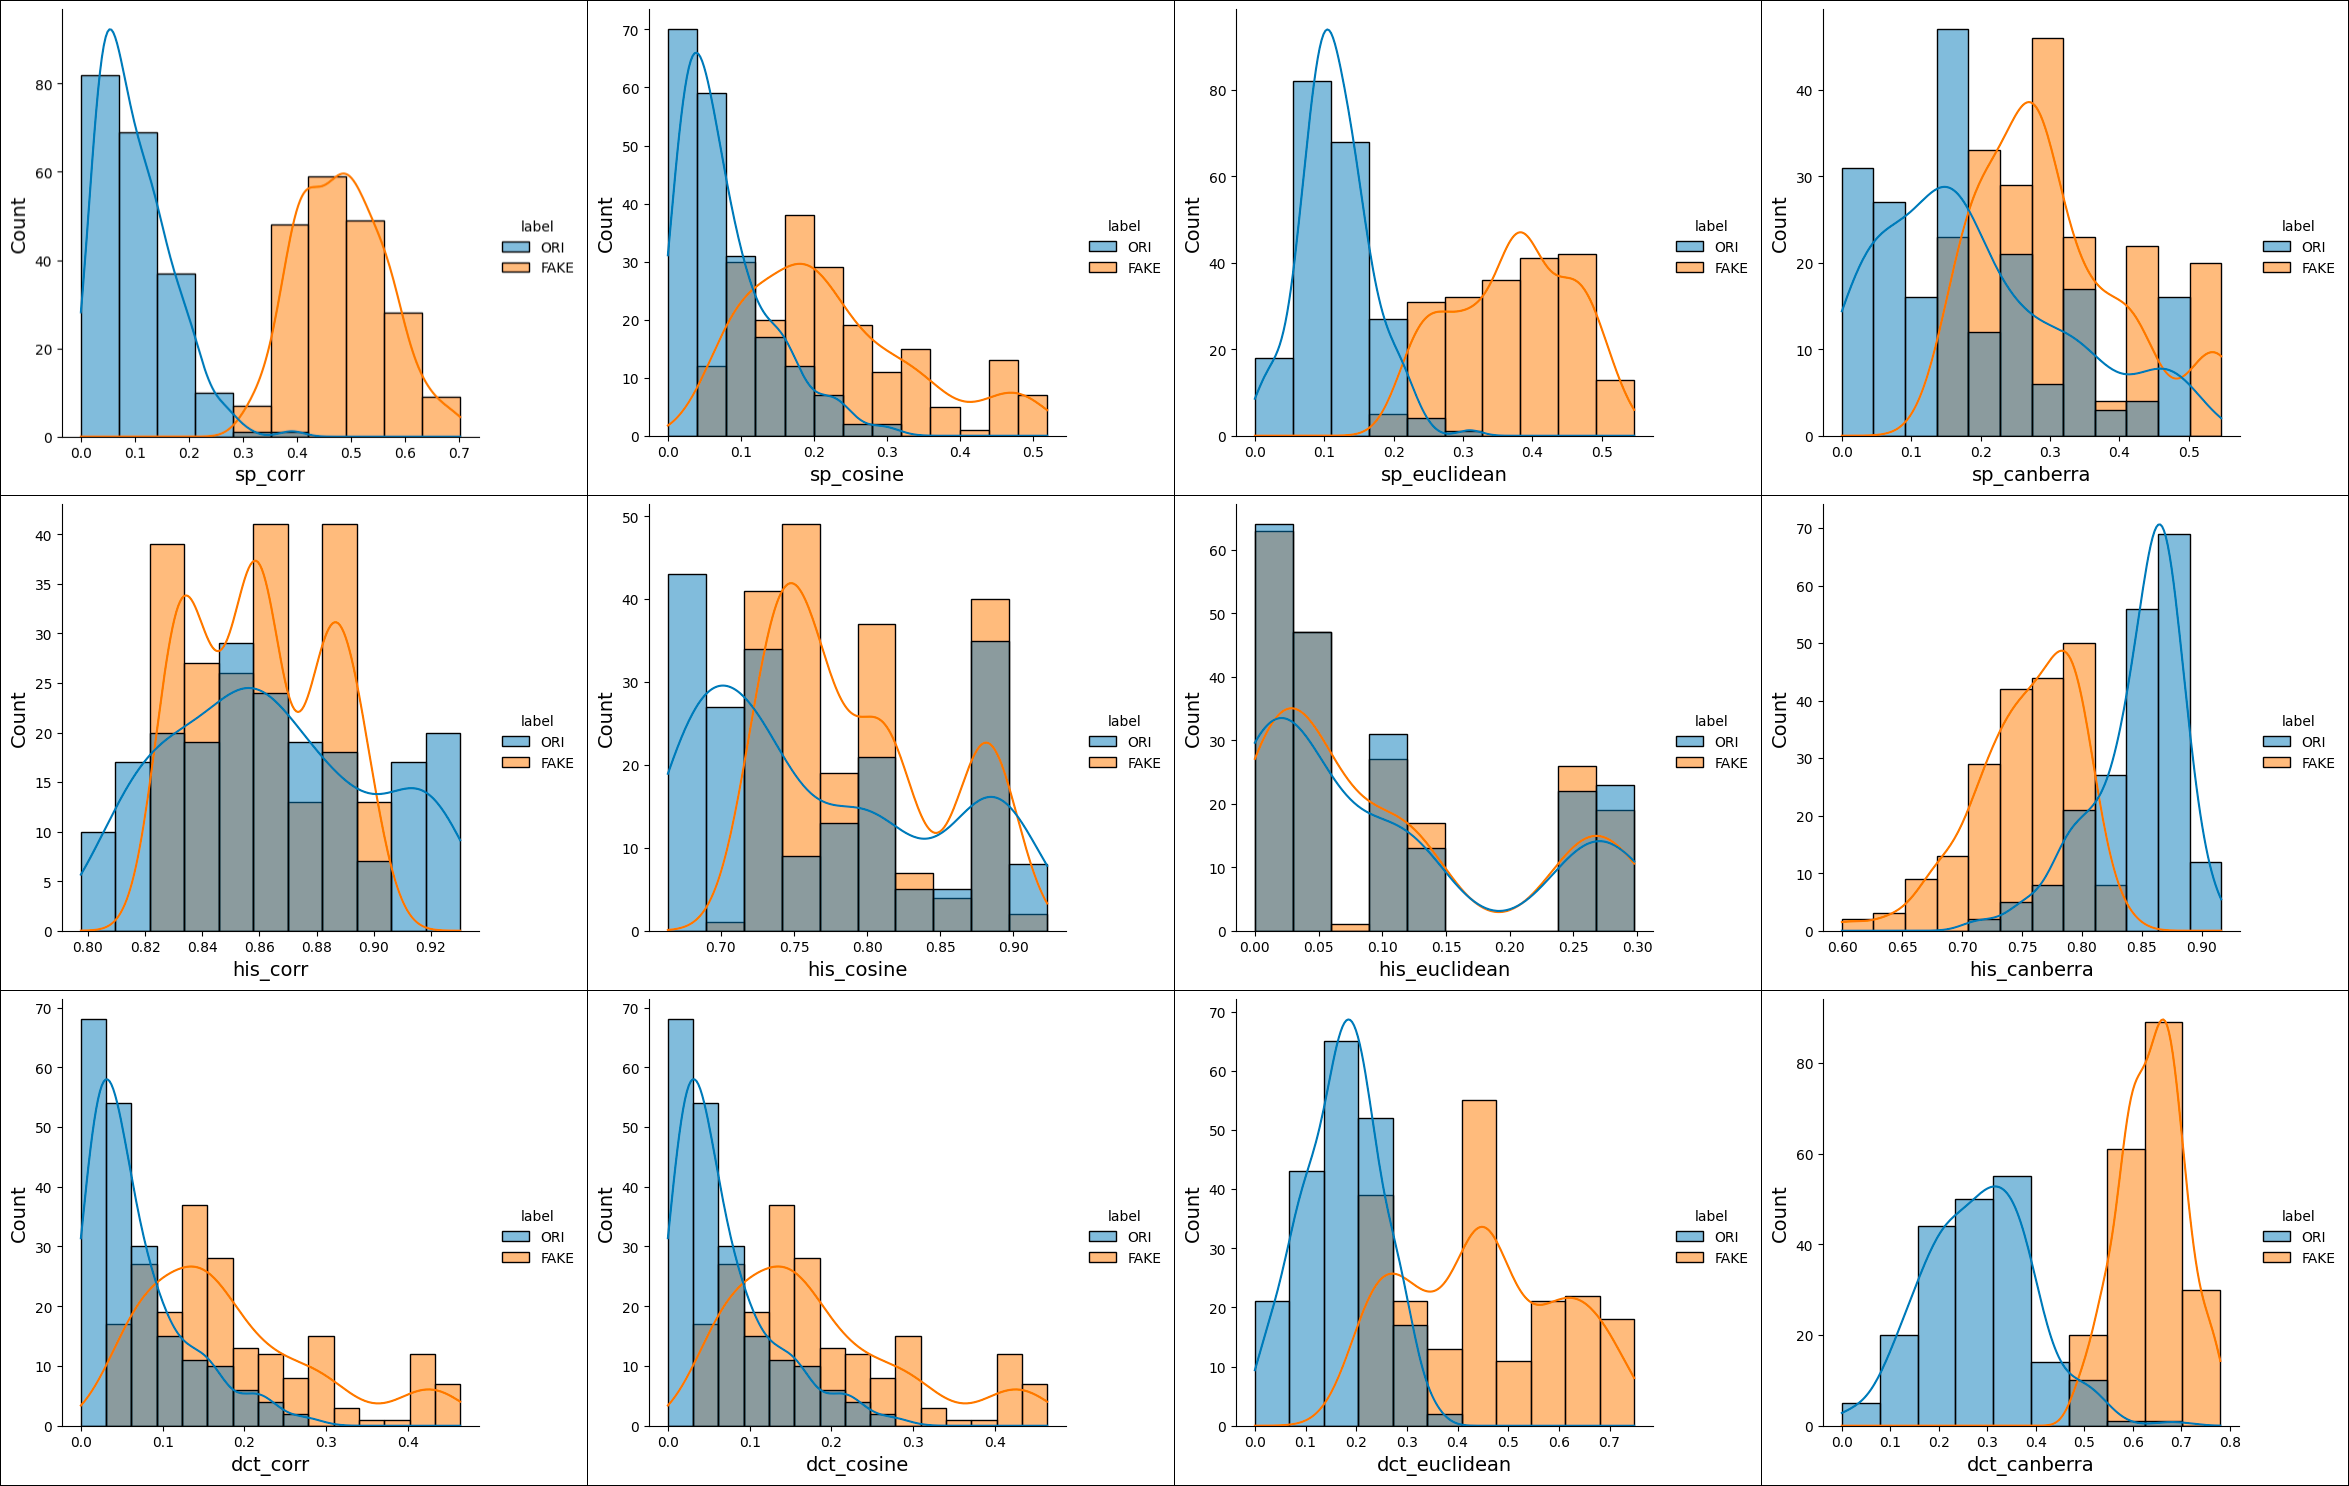
\includegraphics[width=\textwidth]{contents/chapter-4/4-2levelorivs2levelfake.png}
% 	\caption{Plot distribusi koefisien jarak CDP 2 level orisinal dan palsu}
% 	\label{Fig: 4-2levelorivs2levelfake}
% \end{figure}

\clearpage

\begin{figure}[!h]
	\centering
	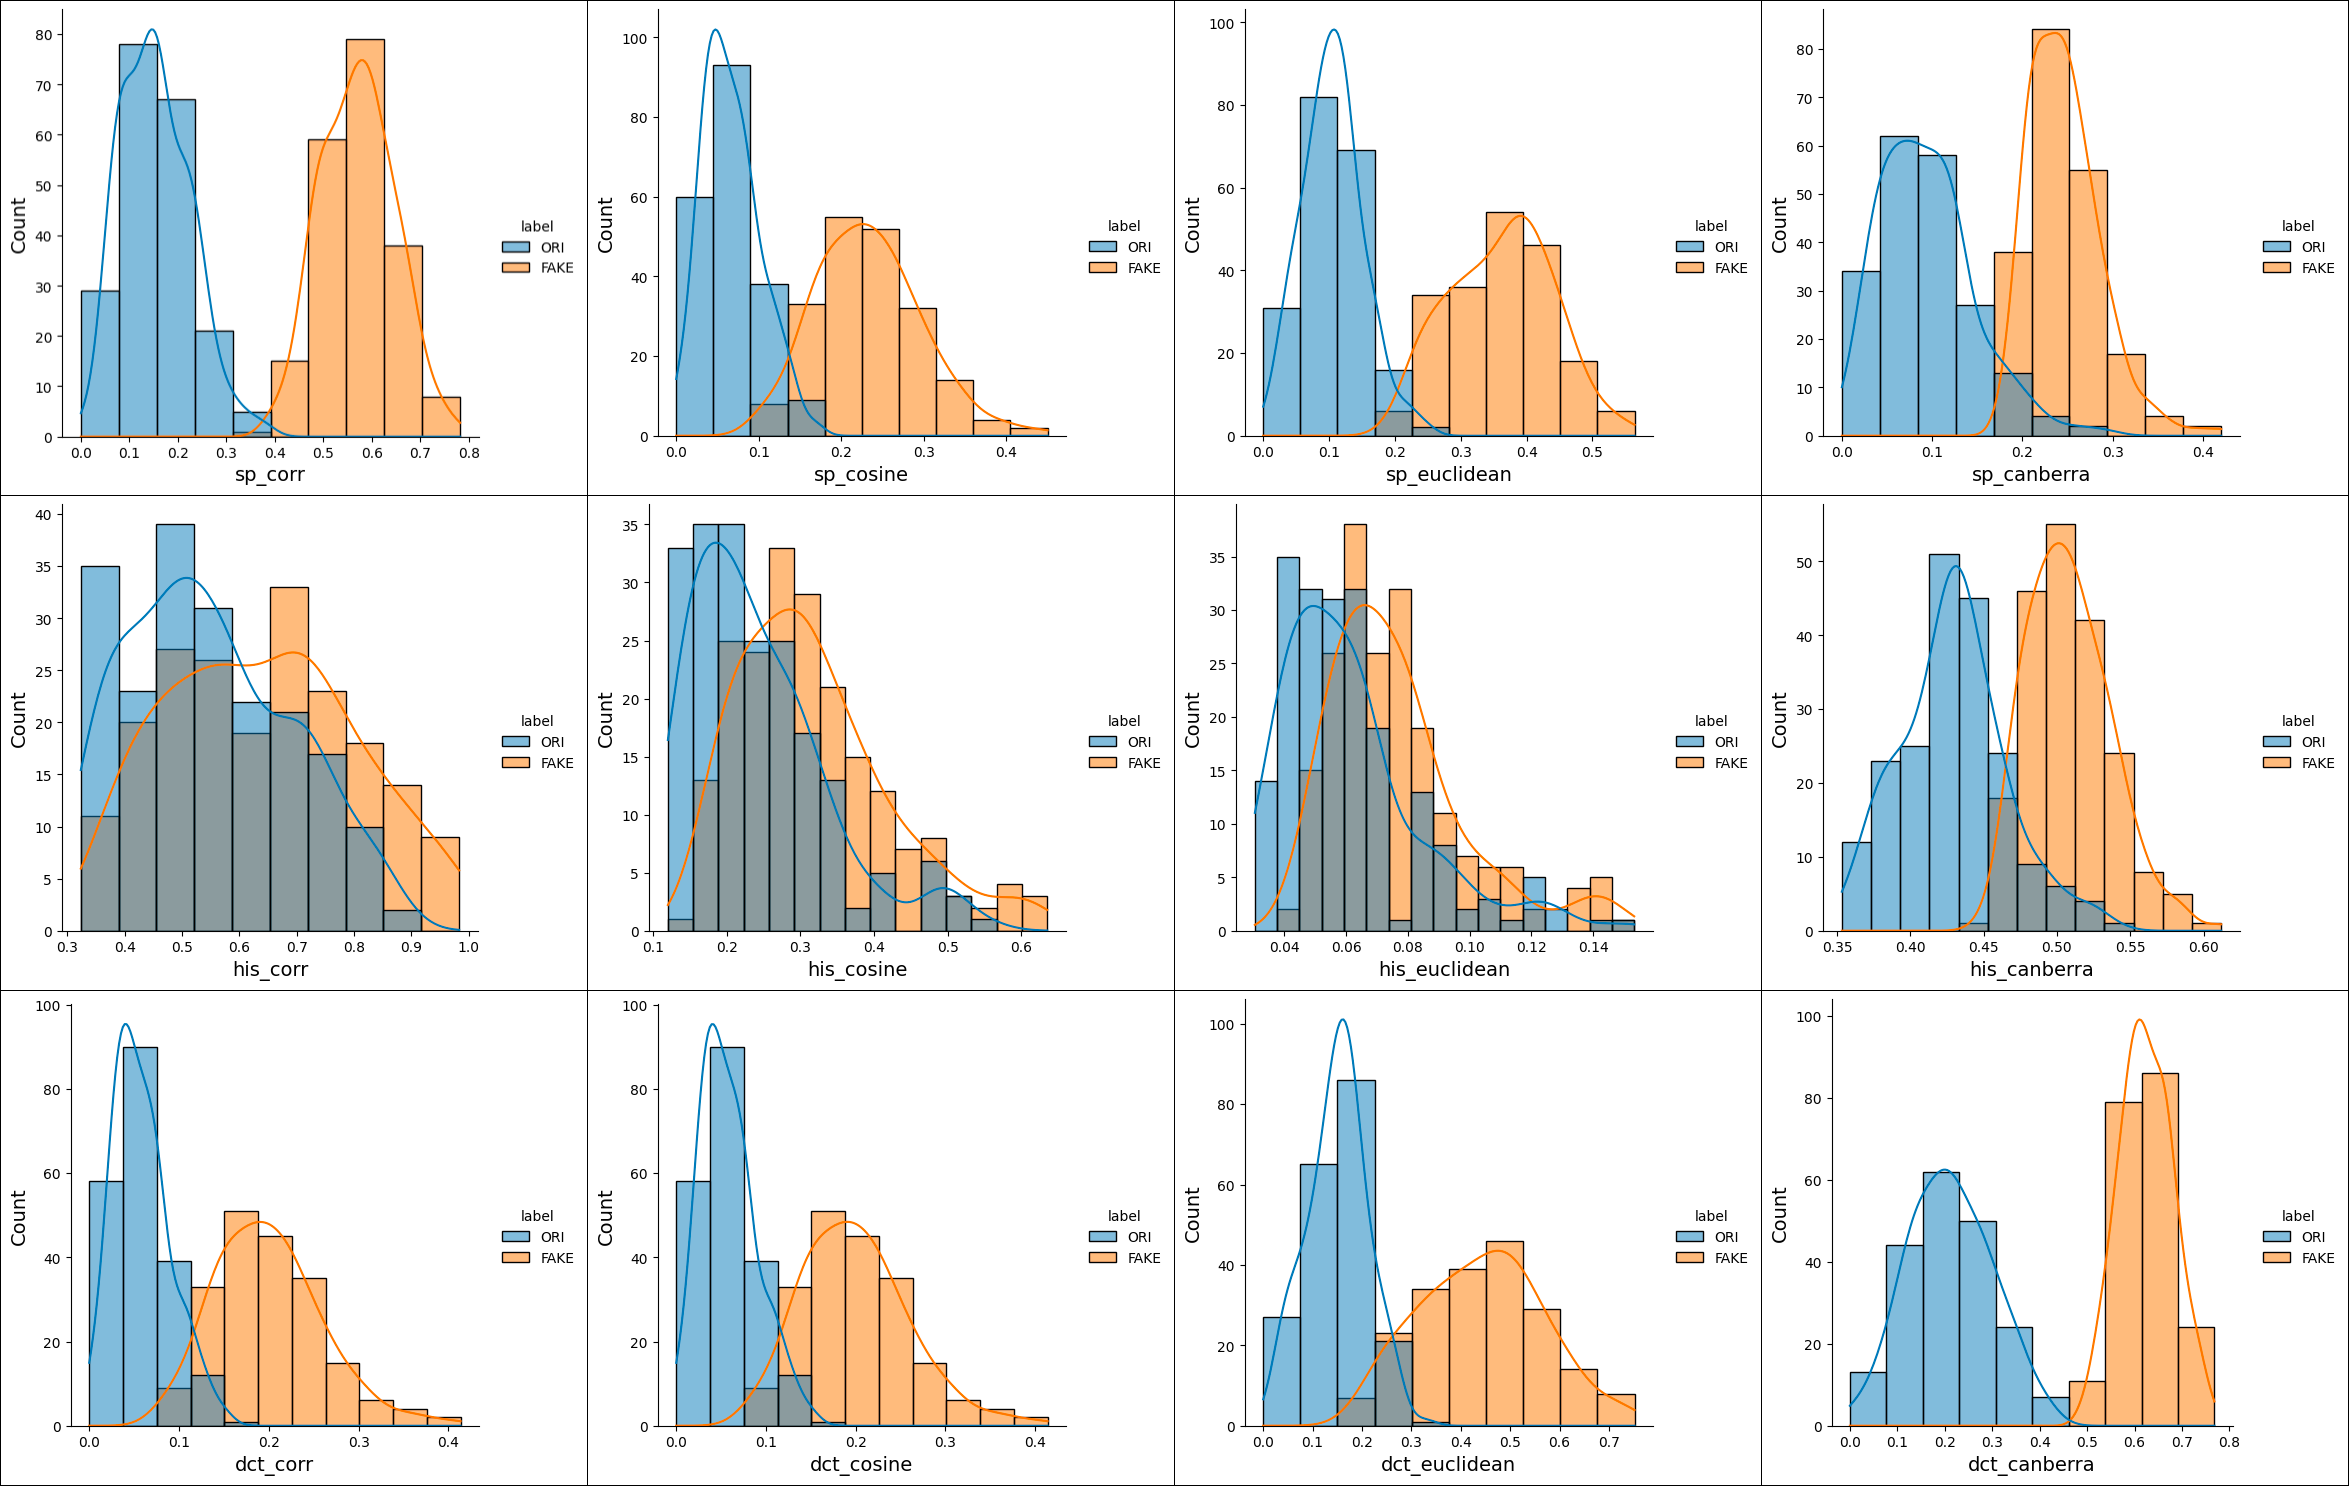
\includegraphics[width=\textwidth]{contents/chapter-4/4-4levelorivs4levelfake.png}
	\caption{Plot distribusi koefisien jarak pada CDP 4 level yang dilokalisasi dengan 8 titik}
	\label{Fig: 4-4levelorivs4levelfake}
\end{figure}

\begin{figure}[!h]
	\centering
	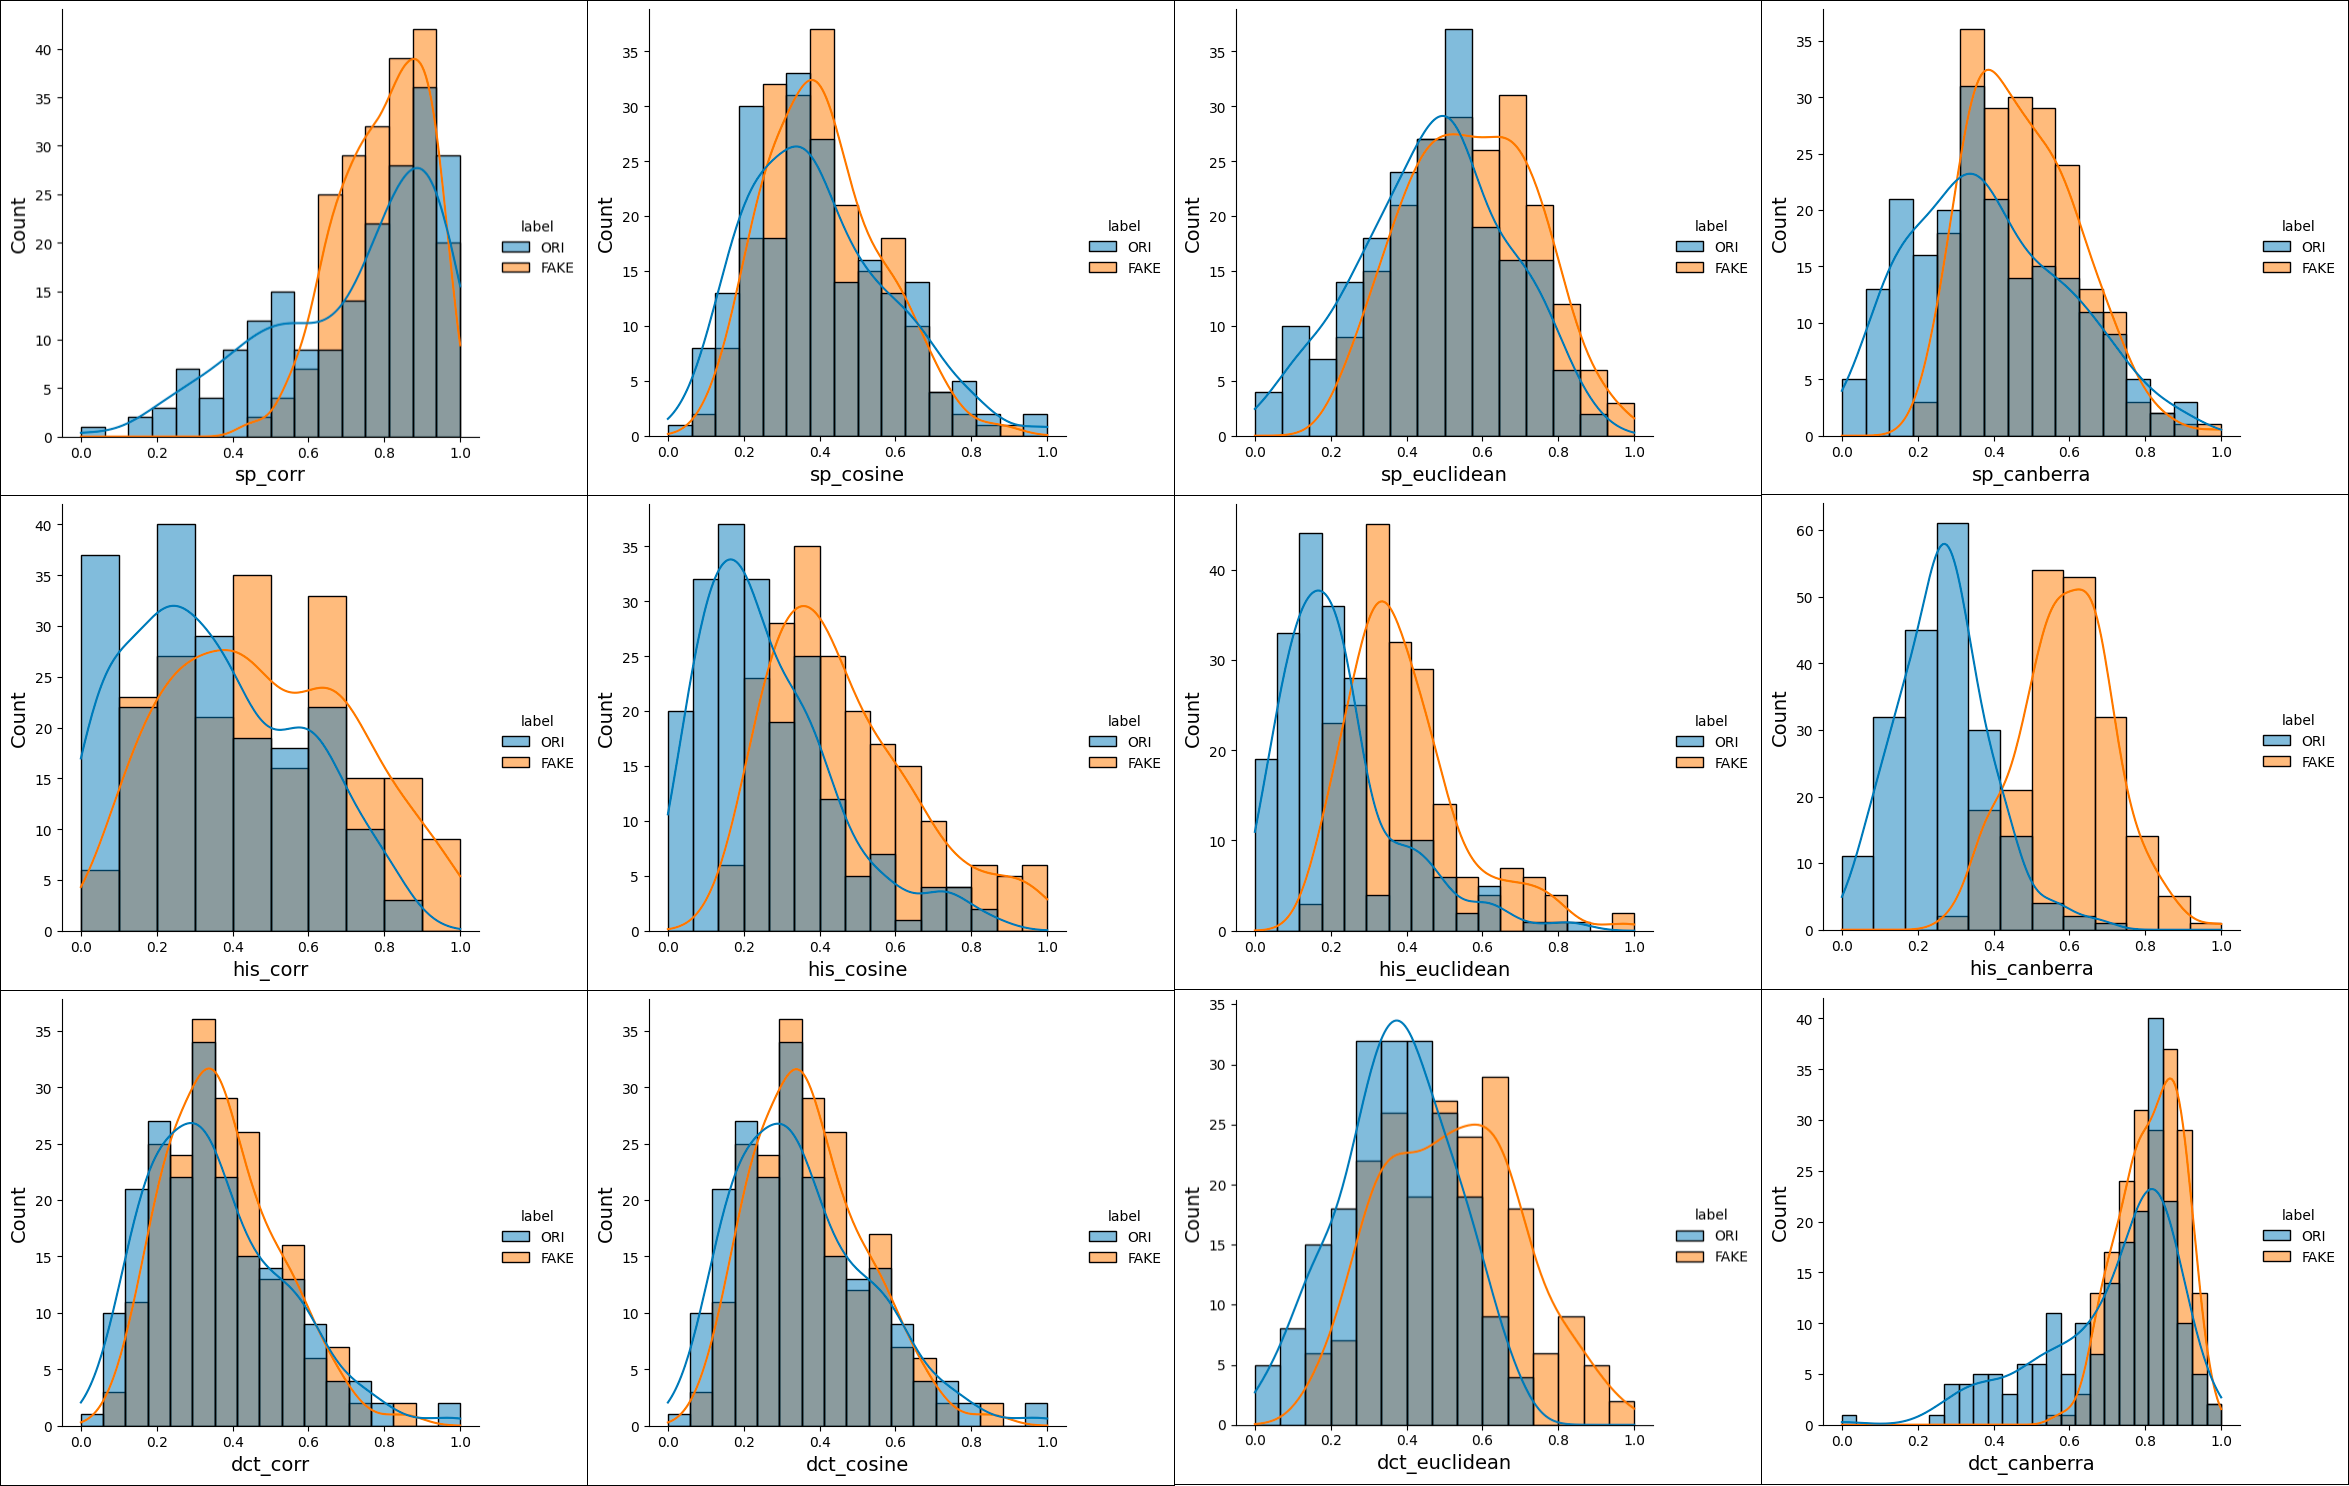
\includegraphics[width=\textwidth]{contents/chapter-4/4-orivsfake4titik.png}
	\caption{Plot distribusi koefisien jarak pada CDP 4 level yang dilokalisasi dengan 4 titik}
	\label{Fig: 4-orivsfake4titik}
\end{figure}

\clearpage

% Selanjutnya untuk hasil plot distribusi \emph{dataset} CDP 4 level dapat dilihat pada \ref{Fig: 4-4levelorivs4levelfake}. Terlihat bahwa hasilnya mirip bahkan
% hampir sama dengan plot distribusi pada \emph{dataset} CDP 2 level. Fitur \emph{sp\_corr} menjadi fitur paling baik yang memisahkan CDP orisinal dan palsu .
% Selain itu, fitur \emph{dct\_canberra} juga memiliki signifikansi yang tinggi. Secara umum analisis fitur jarak menghasilkan hasil yang baik, yaitu mayoritas
% fitur jarak mampu memisahkan CDP orisinal dan palsu, sehingga sangat mungkin hasil model klasifikasi biner yang dibuat memiliki tingkat akurasi yang tinggi
% karena fitur yang digunakan untuk pelatihan sangat berkualitas.

\section{Hasil Pemodelan Klasifikasi Biner}
Pemodelan dilakukan menggunakan dua metode, pertama menggunakan fitur tunggal dari tiap-tiap koefisien jarak, kedua menggunakan multifitur seluruh fitur
koefisien jarak. Akurasi yang dibandingkan adalah akurasi klasifikasi biner pada \emph{dataset} CDP yang dilokalisasi dengan 8 titik dengan \emph{dataset} yang
dilokalisasi dengan 4 titik.

\subsection{Fitur Tunggal}
Untuk menguji performa fitur dalam model, penulis menggunakan semua fitur koefisien jarak satu per satu, baik fitur spasial, histogram, ataupun dct. Model
dibuat dengan AutoGluon dengan memilih model dengan akurasi tertinggi pada data tes. Hasil akurasi klasifikasi biner oleh model dalam mengklasifikasikan SQR
orisinal atau palsu dapat dilihat pada Tabel \ref{Tab: 4-hasilfiturtunggal}.

\begin{table}[!ht]
	\centering
	\caption{Hasil akurasi model klasifikasi biner menggunakan fitur tunggal}
	\vspace{0.5em}
	\begin{tabular}{|l|rr|}
		\hline
		\multirow{2}{*}{}       & \multicolumn{2}{c|}{\textbf{Akurasi}}                                          \\ \cline{2-3}
		                        & \multicolumn{1}{c|}{\textbf{8 Titik}}  & \multicolumn{1}{c|}{\textbf{4 Titik}} \\ \hline
		\textbf{sp\_corr}       & \multicolumn{1}{r|}{\textbf{100.00\%}} & 71.67\%                               \\ \hline
		\textbf{sp\_cosine}     & \multicolumn{1}{r|}{\textbf{94.17\%}}  & 60.83\%                               \\ \hline
		\textbf{sp\_euclidean}  & \multicolumn{1}{r|}{\textbf{98.33\%}}  & 65.00\%                               \\ \hline
		\textbf{sp\_canberra}   & \multicolumn{1}{r|}{\textbf{95.83\%}}  & 68.33\%                               \\ \hline
		\textbf{his\_corr}      & \multicolumn{1}{r|}{57.50\%}           & \textbf{65.00\%}                      \\ \hline
		\textbf{his\_cosine}    & \multicolumn{1}{r|}{69.17\%}           & \textbf{75.00\%}                      \\ \hline
		\textbf{his\_euclidean} & \multicolumn{1}{r|}{69.17\%}           & \textbf{83.33\%}                      \\ \hline
		\textbf{his\_canberra}  & \multicolumn{1}{r|}{90.83\%}           & \textbf{92.50\%}                      \\ \hline
		\textbf{dct\_corr}      & \multicolumn{1}{r|}{\textbf{94.17\%}}  & 55.00\%                               \\ \hline
		\textbf{dct\_cosine}    & \multicolumn{1}{r|}{\textbf{94.17\%}}  & 57.50\%                               \\ \hline
		\textbf{dct\_euclidean} & \multicolumn{1}{r|}{\textbf{94.17\%}}  & 68.33\%                               \\ \hline
		\textbf{dct\_canberra}  & \multicolumn{1}{r|}{\textbf{100.00\%}} & 67.50\%                               \\ \hline
	\end{tabular}
	\label{Tab: 4-hasilfiturtunggal}
\end{table}

Dari hasil yang terlihat pada Tabel \ref{Tab: 4-hasilfiturtunggal}, terlihat bahwa CDP yang dilokalisasi dengan 8 titik memiliki akurasi klasifikasi yang baik
dibandingakan CDP yang dilokalisasi dengan 4 titik. Akurasi tertinggi pada CDP yang dilokalisasi dengan 8 titik didapatkan menggunakan fitur jarak
\emph{sp\_corr} dan \emph{dct\_canberra} dengan akurasi 100\%. Pada CDP yang dilokalisasi dengan 4 titik, akurasi tertinggi didapatkan menggunakan fitur jarak
\emph{his\_canberra} dengan akurasi 92,5\%.

\clearpage

\subsection{Multi Fitur}
\begin{table}[!ht]
	\centering
	\caption{Perbandingan akurasi autentikasi klasifikasi biner pada \emph{dataset} CDP 4 level yang dilokalisasi dengan 8 titik dan \emph{dataset} CDP 4 level yang dilokalisasi dengan 4 titik}
	\vspace{0.5em}
	\begin{tabular}{|cc|cc|}
		\hline
		\multicolumn{2}{|c|}{\textbf{8 titik}} & \multicolumn{2}{c|}{\textbf{4 titik}}                                                                       \\ \hline
		\multicolumn{1}{|c|}{\textbf{Model}}   & \textbf{score\_test}                  & \multicolumn{1}{c|}{\textbf{Model}}  & \textbf{score\_test}         \\ \hline
		\multicolumn{1}{|l|}{XGBoost}          & \multicolumn{1}{r|}{100.00\%}         & \multicolumn{1}{l|}{NeuralNetFastAI} & \multicolumn{1}{r|}{98.33\%} \\ \hline
	\end{tabular}
	\label{Tab: 4-hasilmulti8vs4titik}
\end{table}

Dari hasil yang ditunjukkan pada Tabel \ref{Tab: 4-hasilmulti8vs4titik}, terlihat bahwa akurasi tertinggi yang bisa didapatkan pada \emph{dataset} yang
dilokalisasi dengan 8 titik adalah 100\% menggunakan model XGBoost, sedangkan pada \emph{dataset} yang dilokalisasi dengan 4 titik, akurasi tertinggi yang
didapatkan adalah 98,33\% dengan model NeuralNetFastAI.

Dari hasil-hasil tersebut, baik pembuatan model autentikasi klasifikasi biner menggunakan fitur tunggal atau multi fitur, dapat disimpulkan bahwa
\emph{dataset} yang dilokalisasi dengan 8 titik (dengan bantuan penanda ArUco) memiliki akurasi yang lebih tinggi dibandingkan \emph{dataset} yang dilokalisasi
dengan 4 titik (4 titik sudut kode QR).

% Dari hasil yang terlihat pada Tabel \ref{Tab: 4-hasilfiturtunggal}, terlihat bahwa fitur \emph{sp\_corr} menjadi fitur terbaik dalam pembuatan model
% menggunakan fitur tunggal dengan akurasi 1. Selain itu, pada \emph{dataset} CDP 4 level, fitur \emph{dct\_canberra} juga menghasilkan model dengan akurasi 1.
% Secara mayoritas, akurasi model yang didapatkan oleh \emph{dataset} CDP 4 level lebih baik dari CDP 2 level. CDP 4 level unggul pada 7 fitur sedangkan CDP 2
% level hanya unggul pada 3 fitur. Pada \emph{dataset} CDP 2 level, fitur tunggal yang menghasilkan model dengan akurasi > 0,9 hanya 4 sedangkan pada
% \emph{dataset} CDP 4 level, fitur tunggal yang menghasilkan model dengan akurasi > 0,9 ada 9 fitur.

% \noindent Selanjutnya dapat dilihat pada Tabel \ref{Tab: 4-confusionmatrixfiturtunggal} \emph{confusion matrix} untuk mengetahui \emph{true negative}, \emph{false
% 	positive}, \emph{false negative}, dan \emph{true positive} dari hasil prediksi model.

% % Please add the following required packages to your document preamble:

% \begin{table}[!ht]
% 	\centering
% 	\caption{Hasil \emph{confusion matrix} prediksi model klasifikasi biner menggunakan fitur tunggal}
% 	\vspace{0.5em}
% 	\resizebox{\textwidth}{!}{\begin{tabular}{|c|cc|cc|cc|cc|}
% 			\hline
% 			\multirow{2}{*}{\textbf{}} & \multicolumn{2}{c|}{\textbf{TN}}      & \multicolumn{2}{c|}{\textbf{FP}} & \multicolumn{2}{c|}{\textbf{FN}}      & \multicolumn{2}{c|}{\textbf{TP}}                                                                                                                       \\ \cline{2-9}
% 			                           & \multicolumn{1}{c|}{\textbf{2 Level}} & \textbf{4 Level}                 & \multicolumn{1}{c|}{\textbf{2 Level}} & \textbf{4 Level}                 & \multicolumn{1}{c|}{\textbf{2 Level}} & \textbf{4 Level} & \multicolumn{1}{c|}{\textbf{2 Level}} & \textbf{4 Level} \\ \hline
% 			\textbf{sp\_corr}          & \multicolumn{1}{c|}{60}               & 60                               & \multicolumn{1}{c|}{0}                & 0                                & \multicolumn{1}{c|}{0}                & 0                & \multicolumn{1}{c|}{60}               & 60               \\ \hline
% 			\textbf{sp\_cosine}        & \multicolumn{1}{c|}{55}               & 57                               & \multicolumn{1}{c|}{5}                & 3                                & \multicolumn{1}{c|}{16}               & 4                & \multicolumn{1}{c|}{44}               & 56               \\ \hline
% 			\textbf{sp\_euclidean}     & \multicolumn{1}{c|}{57}               & 60                               & \multicolumn{1}{c|}{3}                & 0                                & \multicolumn{1}{c|}{2}                & 2                & \multicolumn{1}{c|}{58}               & 58               \\ \hline
% 			\textbf{sp\_canberra}      & \multicolumn{1}{c|}{52}               & 60                               & \multicolumn{1}{c|}{8}                & 0                                & \multicolumn{1}{c|}{7}                & 5                & \multicolumn{1}{c|}{53}               & 55               \\ \hline
% 			\textbf{his\_corr}         & \multicolumn{1}{c|}{50}               & 32                               & \multicolumn{1}{c|}{10}               & 28                               & \multicolumn{1}{c|}{22}               & 23               & \multicolumn{1}{c|}{38}               & 37               \\ \hline
% 			\textbf{his\_cosine}       & \multicolumn{1}{c|}{52}               & 47                               & \multicolumn{1}{c|}{8}                & 13                               & \multicolumn{1}{c|}{22}               & 24               & \multicolumn{1}{c|}{38}               & 36               \\ \hline
% 			\textbf{his\_euclidean}    & \multicolumn{1}{c|}{57}               & 54                               & \multicolumn{1}{c|}{3}                & 6                                & \multicolumn{1}{c|}{34}               & 31               & \multicolumn{1}{c|}{26}               & 29               \\ \hline
% 			\textbf{his\_canberra}     & \multicolumn{1}{c|}{59}               & 58                               & \multicolumn{1}{c|}{1}                & 2                                & \multicolumn{1}{c|}{9}                & 9                & \multicolumn{1}{c|}{51}               & 51               \\ \hline
% 			\textbf{dct\_corr}         & \multicolumn{1}{c|}{51}               & 57                               & \multicolumn{1}{c|}{9}                & 3                                & \multicolumn{1}{c|}{15}               & 4                & \multicolumn{1}{c|}{45}               & 56               \\ \hline
% 			\textbf{dct\_cosine}       & \multicolumn{1}{c|}{49}               & 57                               & \multicolumn{1}{c|}{11}               & 3                                & \multicolumn{1}{c|}{14}               & 4                & \multicolumn{1}{c|}{46}               & 56               \\ \hline
% 			\textbf{dct\_euclidean}    & \multicolumn{1}{c|}{49}               & 55                               & \multicolumn{1}{c|}{11}               & 5                                & \multicolumn{1}{c|}{6}                & 2                & \multicolumn{1}{c|}{54}               & 58               \\ \hline
% 			\textbf{dct\_canberra}     & \multicolumn{1}{c|}{60}               & 60                               & \multicolumn{1}{c|}{0}                & 0                                & \multicolumn{1}{c|}{3}                & 0                & \multicolumn{1}{c|}{57}               & 60               \\ \hline
% 		\end{tabular}}
% 	\label{Tab: 4-confusionmatrixfiturtunggal}
% \end{table}

% Setelah melakukan pembuatan model menggunakan fitur tunggal, selanjutnya adalah mencoba pembuatan model menggunakan multi fitur, yaitu seluruh fitur koefisien
% jarak. Dengan penggunaan multi fitur, diharapkan dapat meningkatkan akurasi klasifikasi oleh model. Hasil pembuatan model menggunakan multi fitur pada
% \emph{dataset} CDP 2 level dapat dilihat pada Tabel \ref{Tab: 4-hasilmodel2level}.

% \begin{table}[!ht]
% 	\centering
% 	\caption{Hasil pembuatan model multi fitur pada \emph{dataset} CDP 2 level}
% 	\vspace{0.5em}
% 	\resizebox{\textwidth}{!}{\begin{tabular}{llllll}
% 			\hline
% 			\multicolumn{1}{|c|}{\textbf{Model}} & \multicolumn{1}{c|}{\textbf{score\_test}} & \multicolumn{1}{c|}{\textbf{score\_val}} & \multicolumn{1}{c|}{\textbf{pred\_time\_test}} & \multicolumn{1}{c|}{\textbf{pred\_time\_val}} & \multicolumn{1}{c|}{\textbf{fit\_time}} \\ \hline
% 			\multicolumn{1}{|l|}{LightGBM}       & \multicolumn{1}{r|}{100\%}                & \multicolumn{1}{r|}{100\%}               & \multicolumn{1}{r|}{0.0005}                    & \multicolumn{1}{r|}{0.0007}                   & \multicolumn{1}{r|}{0.2412}             \\ \hline
% 			                                     &                                           &                                          &                                                &                                               &
% 		\end{tabular}}
% 	\label{Tab: 4-hasilmodel2level}
% \end{table}

% \noindent Pada pembuatan model multi fitur menggunakan \emph{dataset} CDP 2 level, hasil akurasi yang diperoleh sangat baik, yaitu 1, baik pada data tes maupun data validasi. Model LightGBM sendiri dipilih berdasarkan urutan pertama dari \emph{leaderboard} yang dikeluarkan oleh AutoGluon yang diurutkan berdasarkan akurasi model pada data tes dan data validasi serta waktu pembuatan model. Untuk hasil pembuatan model menggunakan multi fitur pada \emph{dataset} CDP 4 level dapat dilihat pada Tabel \ref{Tab: 4-hasilmodel4level}.

% \begin{table}[!ht]
% 	\centering
% 	\caption{Hasil pembuatan model multi fitur pada \emph{dataset} CDP 4 level}
% 	\vspace{0.5em}
% 	\resizebox{\textwidth}{!}{\begin{tabular}{llllll}
% 			\hline
% 			\multicolumn{1}{|c|}{\textbf{Model}} & \multicolumn{1}{c|}{\textbf{score\_test}} & \multicolumn{1}{c|}{\textbf{score\_val}} & \multicolumn{1}{c|}{\textbf{pred\_time\_test}} & \multicolumn{1}{c|}{\textbf{pred\_time\_val}} & \multicolumn{1}{c|}{\textbf{fit\_time}} \\ \hline
% 			\multicolumn{1}{|l|}{XGBoost}        & \multicolumn{1}{r|}{100.00\%}             & \multicolumn{1}{r|}{100.00\%}            & \multicolumn{1}{r|}{0.004}                     & \multicolumn{1}{r|}{0.0013}                   & \multicolumn{1}{r|}{0.0722}             \\ \hline
% 			                                     &                                           &                                          &                                                &                                               &
% 		\end{tabular}}
% 	\label{Tab: 4-hasilmodel4level}
% \end{table}

% Dari kedua \emph{dataset}, baik 2 level maupun 4 level, model klasifikasi biner mampu mendapatkan akurasi sempurna, dengan model LightGBM pada CDP 2 level dan
% XGBoost pada CDP 4 level. Selain itu, model AutoGluon juga mencoba beberapa model lain yang telah diurutkan menjadi sebuah \emph{leaderboard}. Hal ini dapat
% memudahkan pengembang model untuk memilih model terbaik dalam kasus yang mereka selesaikan. Untuk perbandingan hasil \emph{leaderboard} model antara CDP 2 dan
% 4 level dapat dilihat pada Tabel \ref{Tab: 4-perbandinganleaderboard2vs4level}.

% \begin{table}[!ht]
% 	\centering
% 	\caption{Perbandingan \emph{leaderboard} model autentikasi pada CDP 2 dan 4 level menggunakan multi fitur}
% 	\vspace{0.5em}
% 	\resizebox{\textwidth}{!}{\begin{tabular}{|lrr|lrr|}
% 			\hline
% 			\multicolumn{3}{|c|}{\textbf{2 Level}}     & \multicolumn{3}{c|}{\textbf{4 Level}}                                                                                                                                                                                   \\ \hline
% 			\multicolumn{1}{|c|}{\textbf{Model}}       & \multicolumn{1}{c|}{\textbf{score\_test}} & \multicolumn{1}{c|}{\textbf{score\_val}} & \multicolumn{1}{c|}{\textbf{Model}}       & \multicolumn{1}{c|}{\textbf{score\_test}} & \multicolumn{1}{c|}{\textbf{score\_val}} \\ \hline
% 			\multicolumn{1}{|l|}{LightGBM}             & \multicolumn{1}{r|}{100.00\%}             & 100.00\%                                 & \multicolumn{1}{l|}{XGBoost}              & \multicolumn{1}{r|}{100.00\%}             & 100.00\%                                 \\ \hline
% 			\multicolumn{1}{|l|}{LightGBMLarge}        & \multicolumn{1}{r|}{100.00\%}             & 100.00\%                                 & \multicolumn{1}{l|}{CatBoost}             & \multicolumn{1}{r|}{100.00\%}             & 100.00\%                                 \\ \hline
% 			\multicolumn{1}{|l|}{LightGBMXT}           & \multicolumn{1}{r|}{100.00\%}             & 100.00\%                                 & \multicolumn{1}{l|}{WeightedEnsemble\_L2} & \multicolumn{1}{r|}{100.00\%}             & 100.00\%                                 \\ \hline
% 			\multicolumn{1}{|l|}{CatBoost}             & \multicolumn{1}{r|}{100.00\%}             & 100.00\%                                 & \multicolumn{1}{l|}{NeuralNetTorch}       & \multicolumn{1}{r|}{100.00\%}             & 100.00\%                                 \\ \hline
% 			\multicolumn{1}{|l|}{WeightedEnsemble\_L2} & \multicolumn{1}{r|}{100.00\%}             & 100.00\%                                 & \multicolumn{1}{l|}{KNeighborsDist}       & \multicolumn{1}{r|}{100.00\%}             & 100.00\%                                 \\ \hline
% 			\multicolumn{1}{|l|}{KNeighborsDist}       & \multicolumn{1}{r|}{100.00\%}             & 100.00\%                                 & \multicolumn{1}{l|}{NeuralNetFastAI}      & \multicolumn{1}{r|}{100.00\%}             & 100.00\%                                 \\ \hline
% 			\multicolumn{1}{|l|}{XGBoost}              & \multicolumn{1}{r|}{100.00\%}             & 100.00\%                                 & \multicolumn{1}{l|}{KNeighborsUnif}       & \multicolumn{1}{r|}{100.00\%}             & 100.00\%                                 \\ \hline
% 			\multicolumn{1}{|l|}{NeuralNetTorch}       & \multicolumn{1}{r|}{100.00\%}             & 100.00\%                                 & \multicolumn{1}{l|}{ExtraTreesEntr}       & \multicolumn{1}{r|}{100.00\%}             & 100.00\%                                 \\ \hline
% 			\multicolumn{1}{|l|}{KNeighborsUnif}       & \multicolumn{1}{r|}{100.00\%}             & 100.00\%                                 & \multicolumn{1}{l|}{ExtraTreesGini}       & \multicolumn{1}{r|}{100.00\%}             & 100.00\%                                 \\ \hline
% 			\multicolumn{1}{|l|}{ExtraTreesEntr}       & \multicolumn{1}{r|}{100.00\%}             & 100.00\%                                 & \multicolumn{1}{l|}{RandomForestEntr}     & \multicolumn{1}{r|}{100.00\%}             & 100.00\%                                 \\ \hline
% 			\multicolumn{1}{|l|}{ExtraTreesGini}       & \multicolumn{1}{r|}{100.00\%}             & 100.00\%                                 & \multicolumn{1}{l|}{RandomForestGini}     & \multicolumn{1}{r|}{100.00\%}             & 100.00\%                                 \\ \hline
% 			\multicolumn{1}{|l|}{RandomForestEntr}     & \multicolumn{1}{r|}{99.17\%}              & 100.00\%                                 & \multicolumn{1}{l|}{LightGBMXT}           & \multicolumn{1}{r|}{99.17\%}              & 100.00\%                                 \\ \hline
% 		\end{tabular}}
% 	\label{Tab: 4-perbandinganleaderboard2vs4level}
% \end{table}

% \subsection{Analisis Perbandingan Akurasi Model pada CDP yang Dilokalisasi Menggunakan Penanda ArUco dan Tanpa Penanda ArUco}
% Untuk mengetahui efektivitas penggunaan ArUco, terutama pada hasil akurasi autentikasinya, penulis membandingkan penggunaan multi fitur dalam pembuatan model
% yang dibandingkan. Perbandingannya adalah antara CDP yang dilokalisasi menggunakan penanda ArUco (8 titik) dan CDP yang dilokalisasi tanpa menggunakan penanda
% ArUco (4 titik). Perbandingan pertama yang dilakukan adalah antara CDP 2 dan 4 level yang dilokalisasi tanpa menggunakan penanda ArUco.

% \begin{table}[!ht]
% 	\centering
% 	\caption{Perbandingan \emph{leaderboard} model CDP 2 dan 4 level pada \emph{dataset} CDP yang dilokalisasi tanpa penanda ArUco}
% 	\vspace{0.5em}
% 	\resizebox{\textwidth}{!}{\begin{tabular}{|lrr|lrr|}
% 			\hline
% 			\multicolumn{3}{|c|}{\textbf{2 Level}}     & \multicolumn{3}{c|}{\textbf{4 Level}}                                                                                                                                                                                   \\ \hline
% 			\multicolumn{1}{|c|}{\textbf{Model}}       & \multicolumn{1}{c|}{\textbf{score\_test}} & \multicolumn{1}{c|}{\textbf{score\_val}} & \multicolumn{1}{c|}{\textbf{Model}}       & \multicolumn{1}{c|}{\textbf{score\_test}} & \multicolumn{1}{c|}{\textbf{score\_val}} \\ \hline
% 			\multicolumn{1}{|l|}{NeuralNetFastAI}      & \multicolumn{1}{r|}{96.67\%}              & 98.21\%                                  & \multicolumn{1}{l|}{NeuralNetFastAI}      & \multicolumn{1}{r|}{\textbf{98.33\%}}     & \textbf{100.00\%}                        \\ \hline
% 			\multicolumn{1}{|l|}{WeightedEnsemble\_L2} & \multicolumn{1}{r|}{96.67\%}              & 98.21\%                                  & \multicolumn{1}{l|}{WeightedEnsemble\_L2} & \multicolumn{1}{r|}{\textbf{98.33\%}}     & \textbf{100.00\%}                        \\ \hline
% 		\end{tabular}}
% 	\label{Tab: 4-perbandinganleaderboard2vs4leveltanpaaruco}
% \end{table}

% Dari Tabel \ref{Tab: 4-perbandinganleaderboard2vs4leveltanpaaruco} dapat dilihat bahwa hasil akurasi model pada data tes tertinggi yang diperoleh pada
% \emph{dataset} CDP yang dilokalisasi tanpa menggunakan penanda ArUco adalah 0,967 pada CDP 2 level dan 0,983 pada CDP 4 level. Pada data validasi skor
% tertinggi yang diperoleh adalah 0,982 pada CDP 2 level dan 1 pada CDP 4 level. Dari hasil ini didapatkan bahwa hasil lokalisasi CDP menggunakan penanda ArUco
% (8 titik) lebih baik dengan yang tanpa menggunakan penanda ArUco (4 titik), baik dari kemiripinnya dengan \emph{template} ataupun dari akurasi klasifikasi
% biner oleh model. Selain itu, pada \emph{dataset} yang kurang baik (CDP hasil lokalisasi 4 titik), CDP 4 level memiliki hasil akurasi yang lebih baik
% dibandingkan CDP 2 level. Hal tersebut menjawab hipotesis yang dituliskan penulis di awal, yaitu lokalisasi CDP menggunakan penanda ArUco (8 titik) lebih baik
% daripada tanpa penanda ArUco (4 titik) dan CDP dengan 4 level \emph{grayscale} lebih baik untuk digunakan dalam mengautentikasi SQR. Kedua hipotesis tersebut
% terbukti benar dari hasil penelitian yang didapatkan.